% Try doing this with beamer.

\documentclass{beamer}

\providecommand\insertframetitle{} 

\setbeamertemplate{footline}[page number]
\setbeamertemplate{frametitle}{
\begin{center}
\insertframetitle%
\vspace{-2cm}%
\end{center}
}
\setbeamertemplate{navigation symbols}{}
\setbeamercovered{again covered={\opaqueness<1->{40}}}

% Would be nice to know what kind of resolution projector I'm looking at.
% My screen is SVGA, the equivalent of a low-end projector (800x600).
% Next higher resolution is XGA (1024x768), which I would need Laura's computer to try.

%\usefonttheme{serif} % Beamer guide recommends taking a look at futura, but I can't figure out how to pick a font family...
\usepackage{arev}
\renewcommand{\sfdefault}{arev}
%\setbeamerfont{*}{family=arev}

\usepackage{mdframed} % Make custom boxes.
\usepackage{tikz}
\usetikzlibrary{shapes}

\makeatletter
\pgfdeclareshape{PhotonBin}{
\inheritsavedanchors[from=rectangle] % this is nearly a rectangle
%\inheritanchorborder[from=rectangle]
\inheritanchor[from=rectangle]{center}
\inheritanchor[from=rectangle]{north}
\inheritanchor[from=rectangle]{south}
\inheritanchor[from=rectangle]{west}
\inheritanchor[from=rectangle]{east}

\backgroundpath{% this is new
% store lower left in xa/ya and upper right in xb/yb
\southwest \pgf@xa=\pgf@x \pgf@ya=\pgf@y
\northeast \pgf@xb=\pgf@x \pgf@yb=\pgf@y

% construct main path
\pgfpathmoveto{\pgfpoint{\pgf@xa}{\pgf@yb}}
\pgfsetlinewidth{2pt}
\pgfpathlineto{\pgfpoint{\pgf@xa}{\pgf@ya}}
\pgfpathlineto{\pgfpoint{\pgf@xb}{\pgf@ya}}
\pgfpathlineto{\pgfpoint{\pgf@xb}{\pgf@yb}}
}
}
\makeatother

\usepackage{framed} % For boxing things
\usepackage{graphicx} % To include graphics.
\usepackage{enumitem} % For list customizability.
\setitemize{label=\usebeamerfont*{itemize item}% enumitem and beamer conflict; this fixes it.
  \usebeamercolor[fg]{itemize item}
  \usebeamertemplate{itemize item}}

\title{A Search for the Neutrinoless Double Beta
Decay of Xenon-136 with Improved
Sensitivity from Denoising}

\author{Clayton G. Davis}
\date{April 3, 2014}

\begin{document}

\begin{frame}
\titlepage
\end{frame}

\section*{Outline}
\begin{frame}
\frametitle{Outline}
\tableofcontents
\end{frame}

\section{\texorpdfstring{$\beta\beta 2\nu$ and $\beta\beta 0\nu$}{Two-Neutrino and Neutrinoless Double-Beta} Decay}

\begin{frame}
\begin{center}
\frametitle{What is Double-Beta Decay?}
\end{center}
\begin{columns}
\begin{column}{.5\textwidth}
\includegraphics<1>[keepaspectratio=true,height=180pt]{Avignone_fig02a.eps}
\includegraphics<2>[keepaspectratio=true,height=180pt]{Avignone_fig02b.eps}\\
\tiny Avignone et al., RMP 2008.
\end{column}
\begin{column}{.5\textwidth}
\uncover<1>{Feynman diagram for $\beta\beta 2 \nu$ decay.   Equivalent to two single-$\beta$ decays:
\begin{align*}
2n &\rightarrow 2p + 2e^- + 2\bar{\nu}_e \\
\text{eg. } ^{136}\text{Xe} &\rightarrow {}^{136}\text{Ba} + 2e^- + 2\bar{\nu}_e \end{align*} }%
\uncover<2>{Feynman diagram for $\beta\beta 0 \nu$ decay.   Neutrinos annihilate each other:
\begin{align*}
2n &\rightarrow 2p + 2e^- \phantom{{} + 2\bar{\nu}_e}\\
\text{eg. } ^{136}\text{Xe} &\rightarrow {}^{136}\text{Ba} + 2e^- \phantom{{} + 2\bar{\nu}_e} \end{align*}%
$\beta\beta 2 \nu$ is allowed in the Standard Model; $\beta\beta 0 \nu$ is not.}%
\end{column}
\end{columns}
\end{frame}

\begin{frame}
\begin{center}
\frametitle{Implications of Double-Beta Decay}
\end{center}
\begin{columns}
\begin{column}{.5\textwidth}
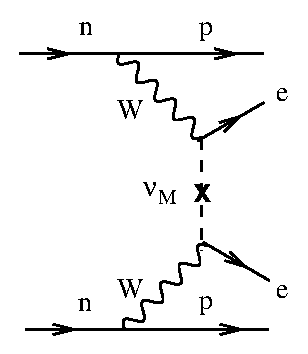
\includegraphics[keepaspectratio=true,height=180pt]{Avignone_fig02b.eps}\\
\tiny Avignone et al., RMP 2008.
\end{column}
\begin{column}{.5\textwidth}
\begin{itemize}
\item Lepton number changes:\[\Delta L = +2\]
\item Neutrinos can convert to their own antiparticle:\[\bar{\nu}_R \rightarrow \nu_L\]
\item Neutrinos have mass through a Majorana interaction:
\[-\frac{m_L}{2}\left(\overline{\Psi^c_L} \Psi_L +  \overline{\Psi_L} \Psi^c_L\right)\]
\[-\frac{m_R}{2}\left(\overline{\Psi^c_R} \Psi_R +  \overline{\Psi_R} \Psi^c_R\right)\]
\end{itemize}
\end{column}
\end{columns}
\end{frame}

\begin{frame}
\begin{center}
\frametitle{The $A=136$ Isobar}
\end{center}
\begin{columns}
\begin{column}{.5\textwidth}
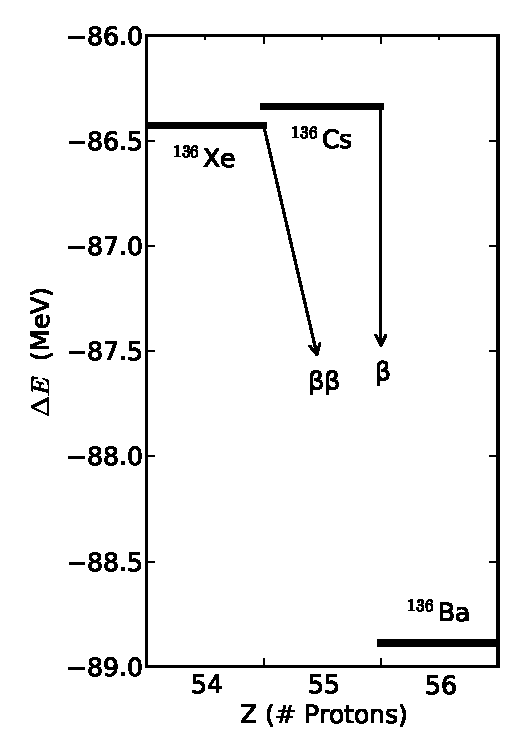
\includegraphics[keepaspectratio=true,width=\textwidth]{LevelDiagram.pdf}\\
\end{column}
\begin{column}{.5\textwidth}
$^{136}$Cs undergoes single-$\beta$ decay.\\[\baselineskip]
$^{136}$Xe cannot, due to energy conservation -- but it can $\beta\beta$ decay through $^{136}$Cs to $^{136}$Ba.\\[\baselineskip]
The $Q$-value of $^{136}\text{Xe}\rightarrow ^{136}\text{Ba}$ is $2457.83 \pm 0.37$ keV, shared between all final products of the decay.\\[\baselineskip]
We observe energy in electrons; energy in neutrinos is lost.
\end{column}
\end{columns}
\end{frame}

\begin{frame}
\begin{center}
\frametitle{Ideal Double-Beta Energy Spectrum}
\end{center}
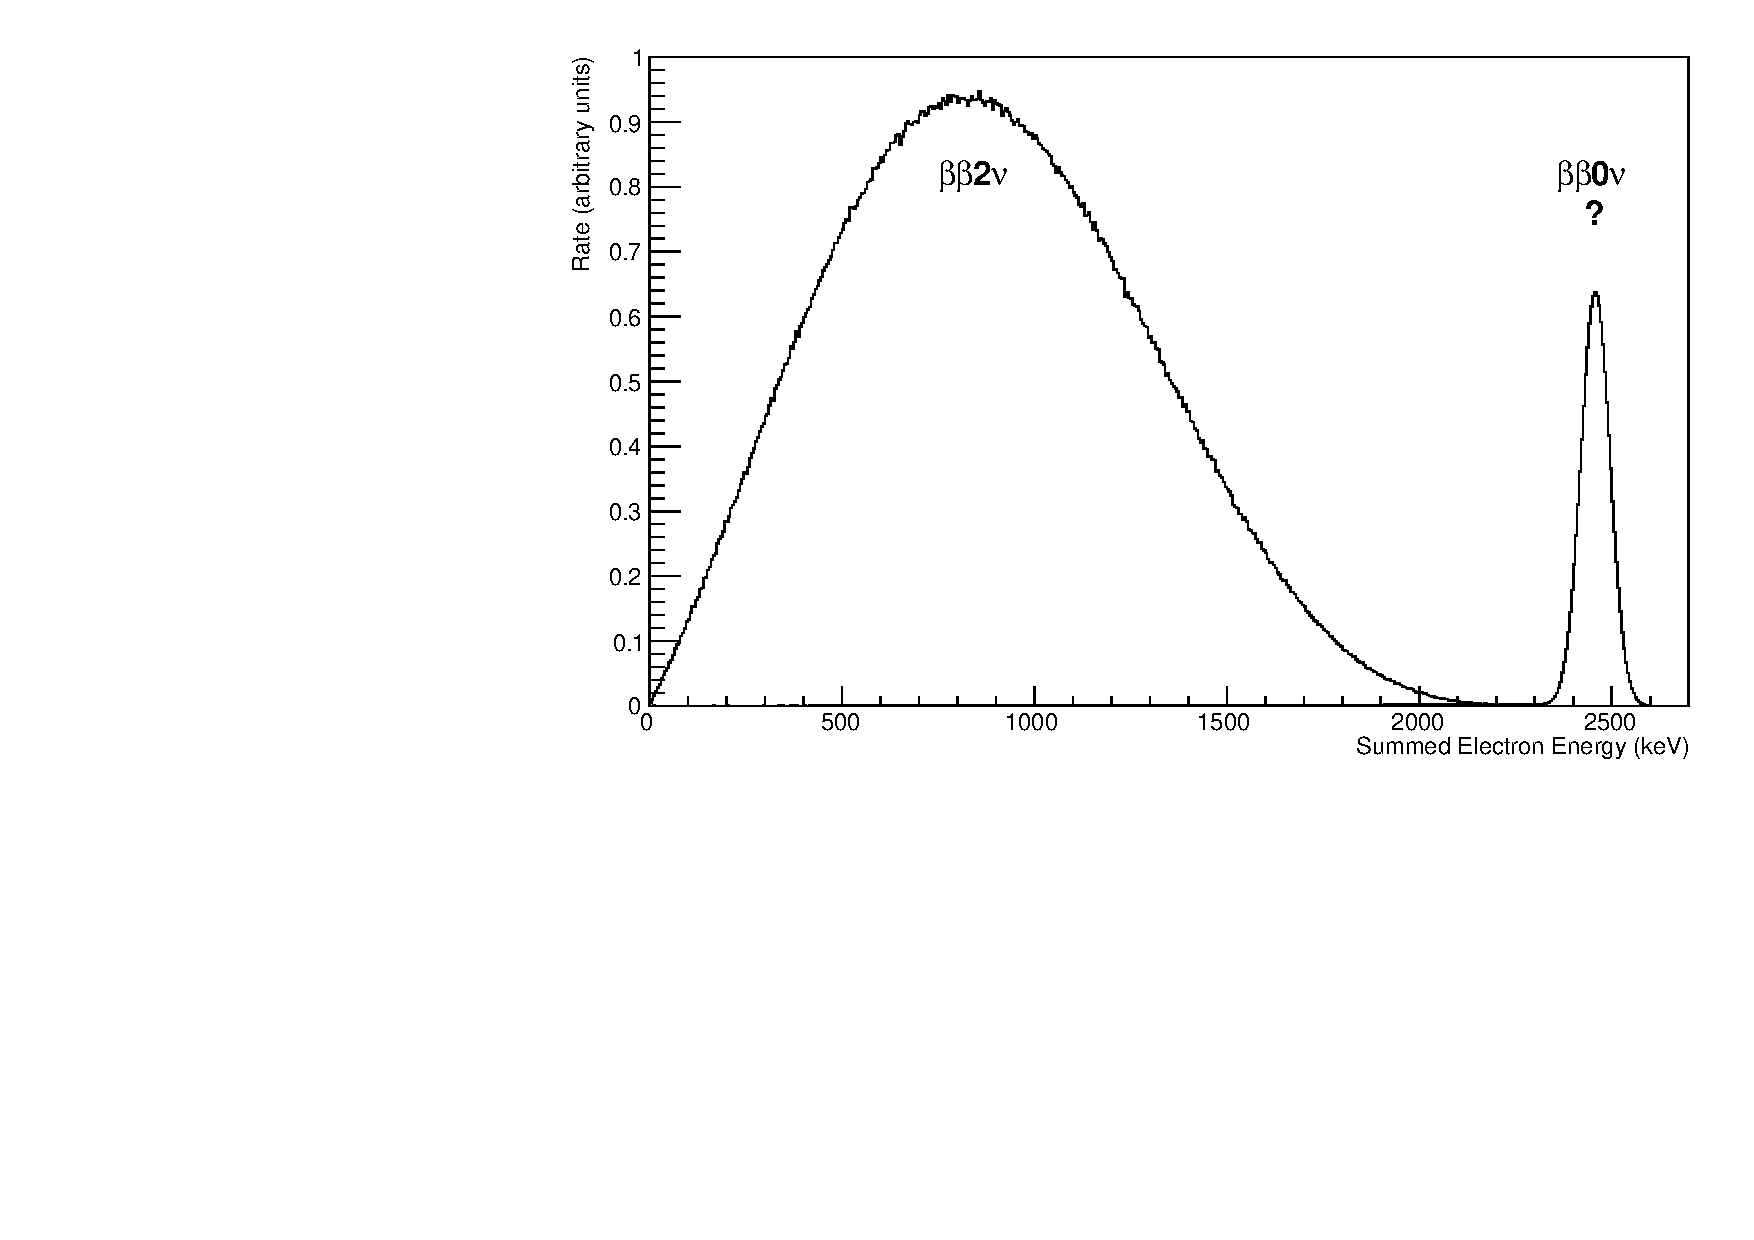
\includegraphics[keepaspectratio=true,width=\textwidth]{IdealSpectrum.pdf}\\
\only<1>{$^{136}$Xe $\beta\beta 2\nu$ produces a smooth energy spectrum; ``missing'' energy carried off by neutrinos.}
\only<2>{$^{136}$Xe $\beta\beta 0\nu$ has no neutrinos, so no ``missing'' energy; mono-energetic peak at $Q = 2458$ keV.}
\only<3>{If the $\beta\beta 0\nu$ peak exists, neutrinos have Majorana mass; peak height gives a measurement of that mass.}
\end{frame}

\begin{frame}
\begin{center}
\frametitle{Observed Double-Beta Energy Spectrum (Previous Result)}
\end{center}
\textcolor{red}{Show previous result spectrum here, as a real example.}
\end{frame}

\section{The EXO-200 Detector}

\begin{frame}
\begin{center}
\frametitle{The EXO-200 Detector}
\end{center}
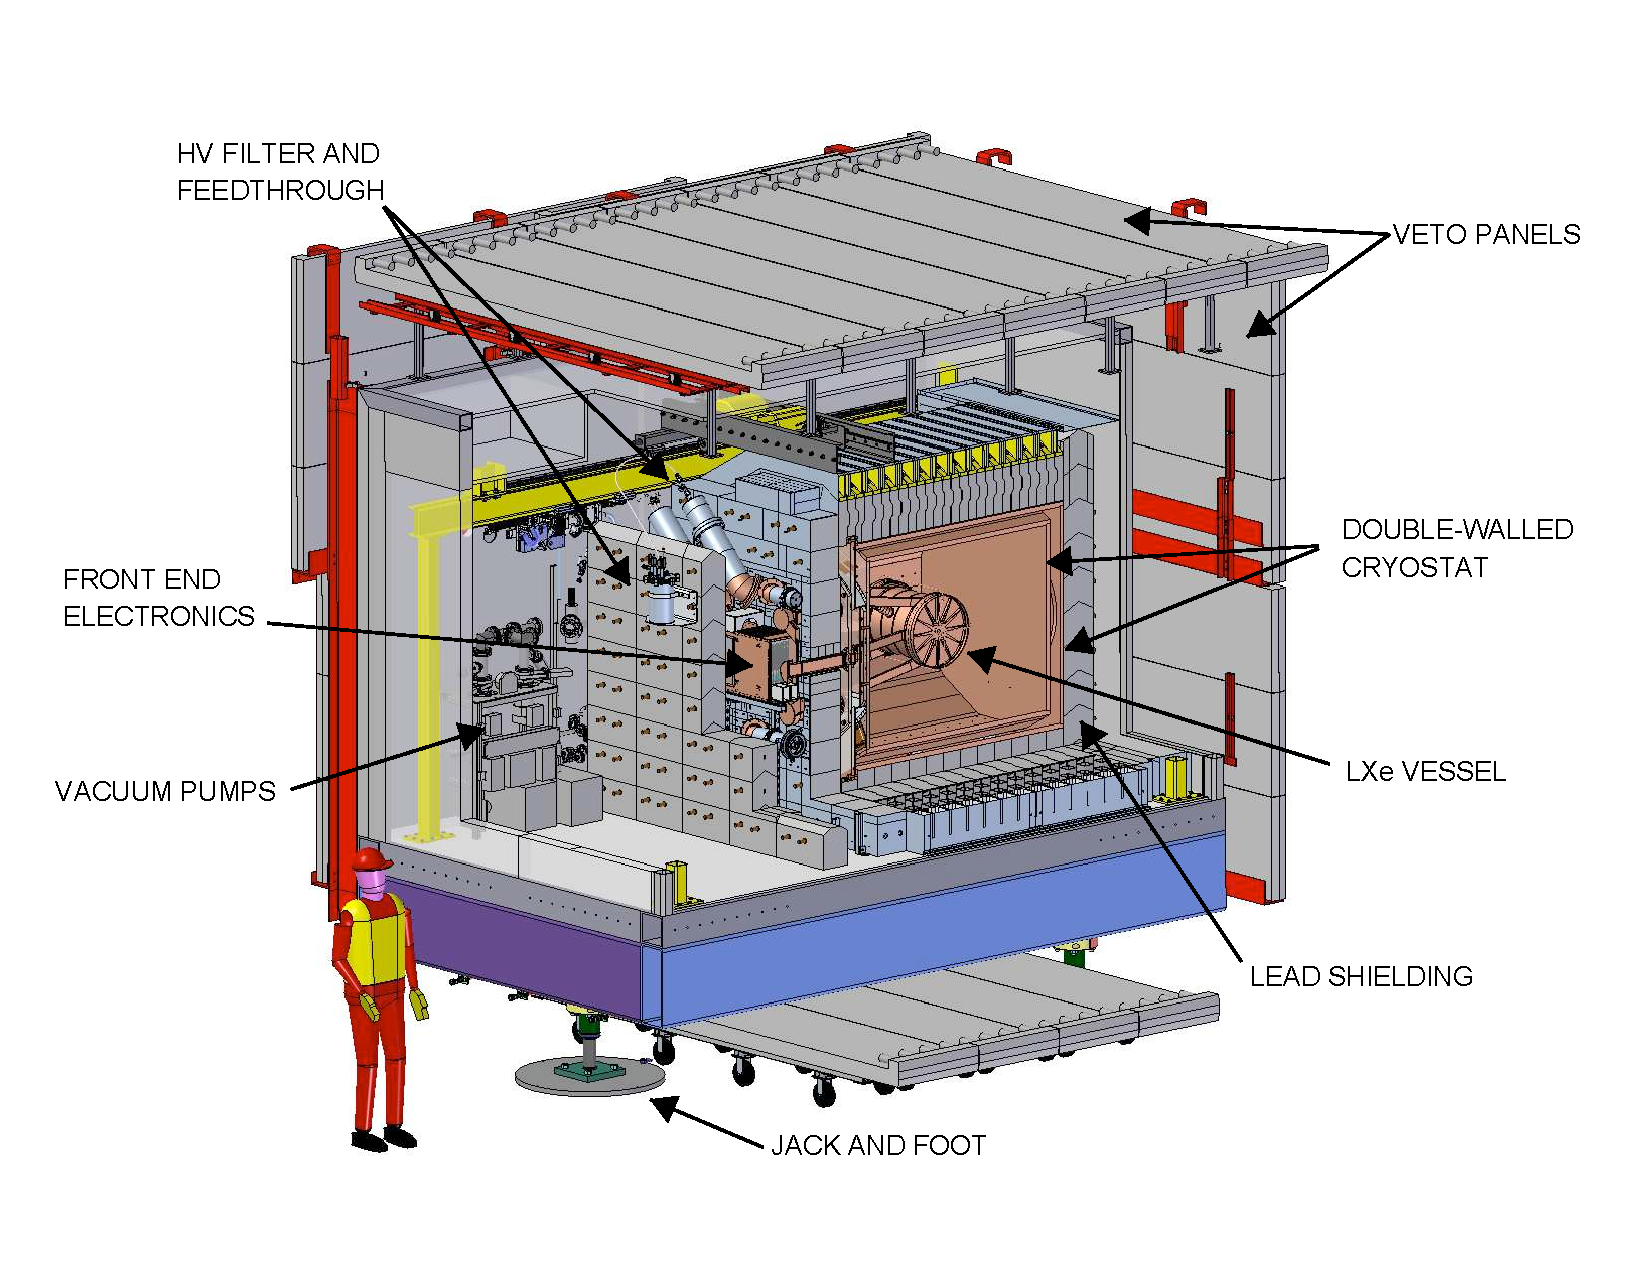
\includegraphics[keepaspectratio=true,width=\textwidth]{cleanroom.pdf}
\end{frame}

\begin{frame}
\begin{center}
\frametitle{The EXO-200 Detector}
\end{center}
\begin{columns}[onlytextwidth]
\begin{column}{.5\textwidth}
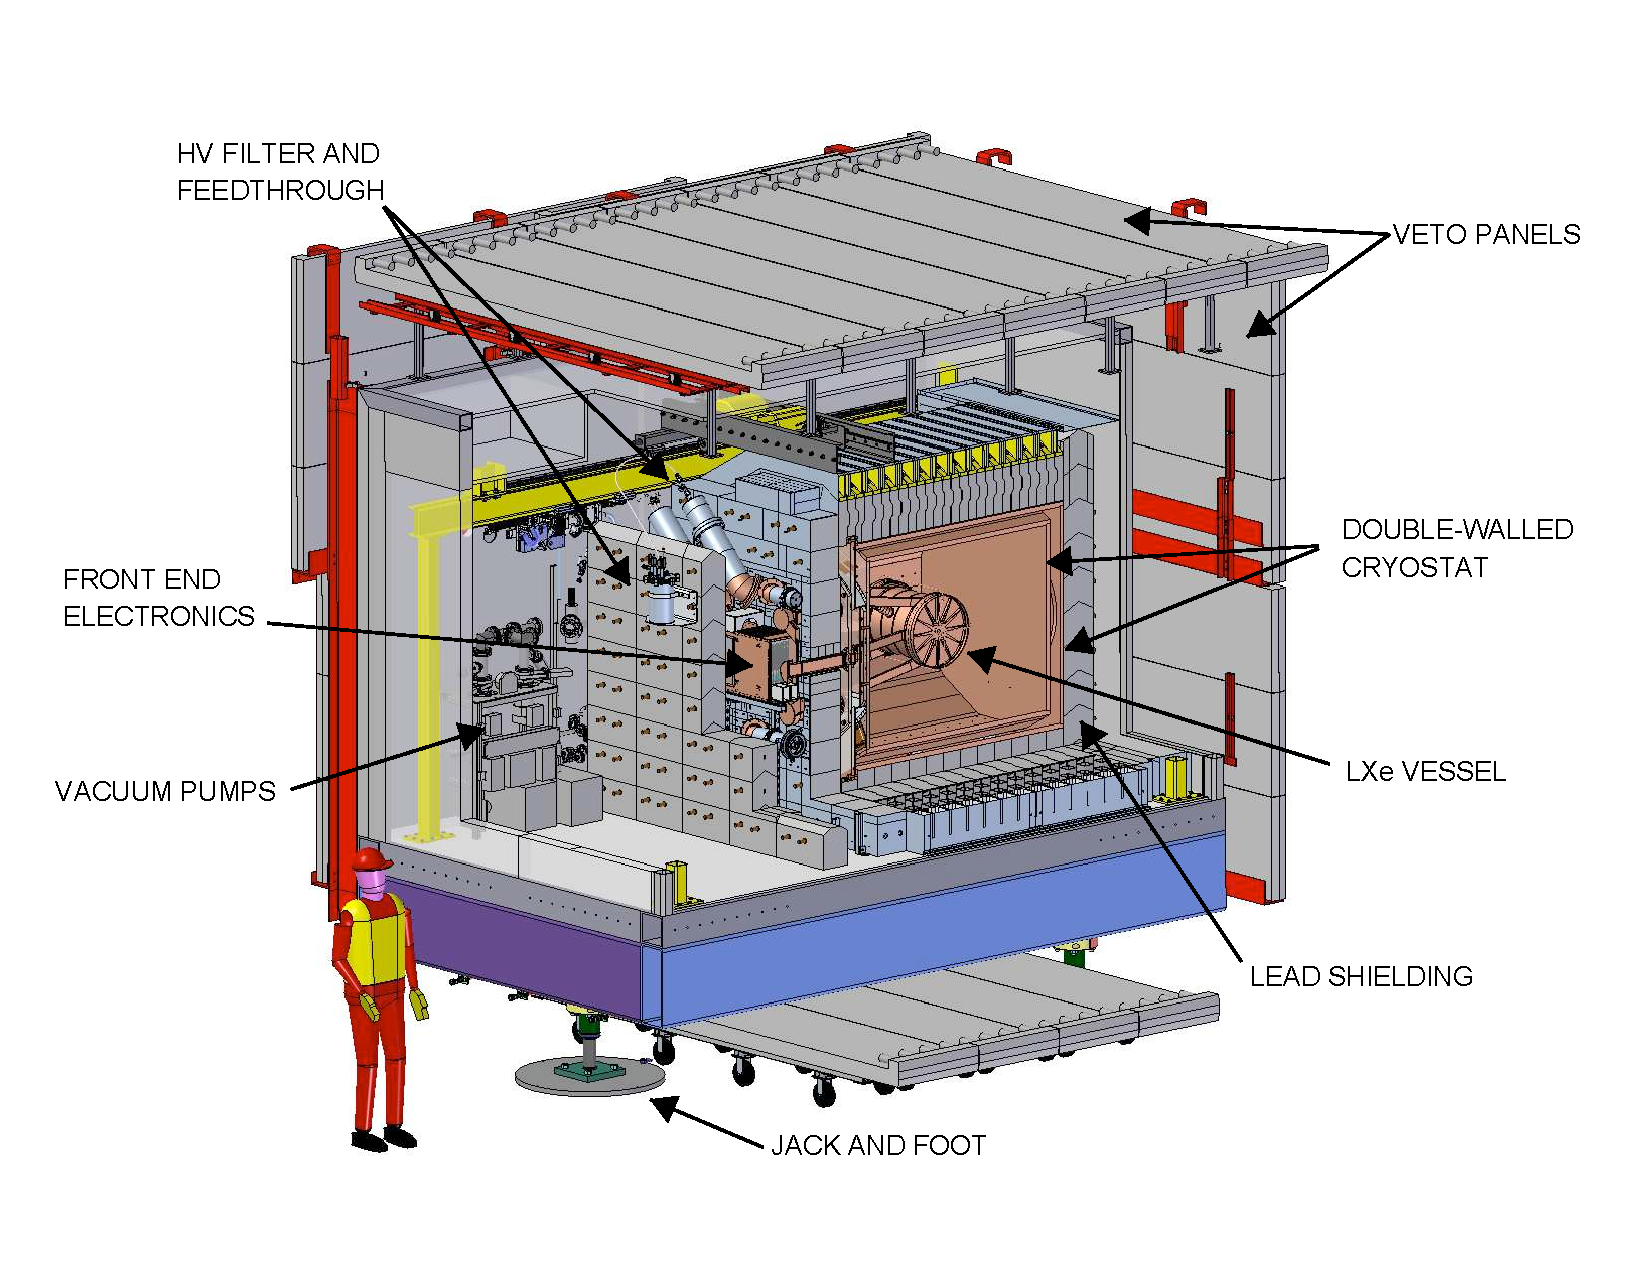
\includegraphics[keepaspectratio=true,width=\textwidth]{cleanroom.pdf}\\
To search for rare decays, low background is key:
\begin{itemize}
\item Clean (low-radioactivity) materials surrounding TPC.
\item Deep underground to avoid cosmogenics.
\end{itemize}
\end{column}
\begin{column}{.5\textwidth}
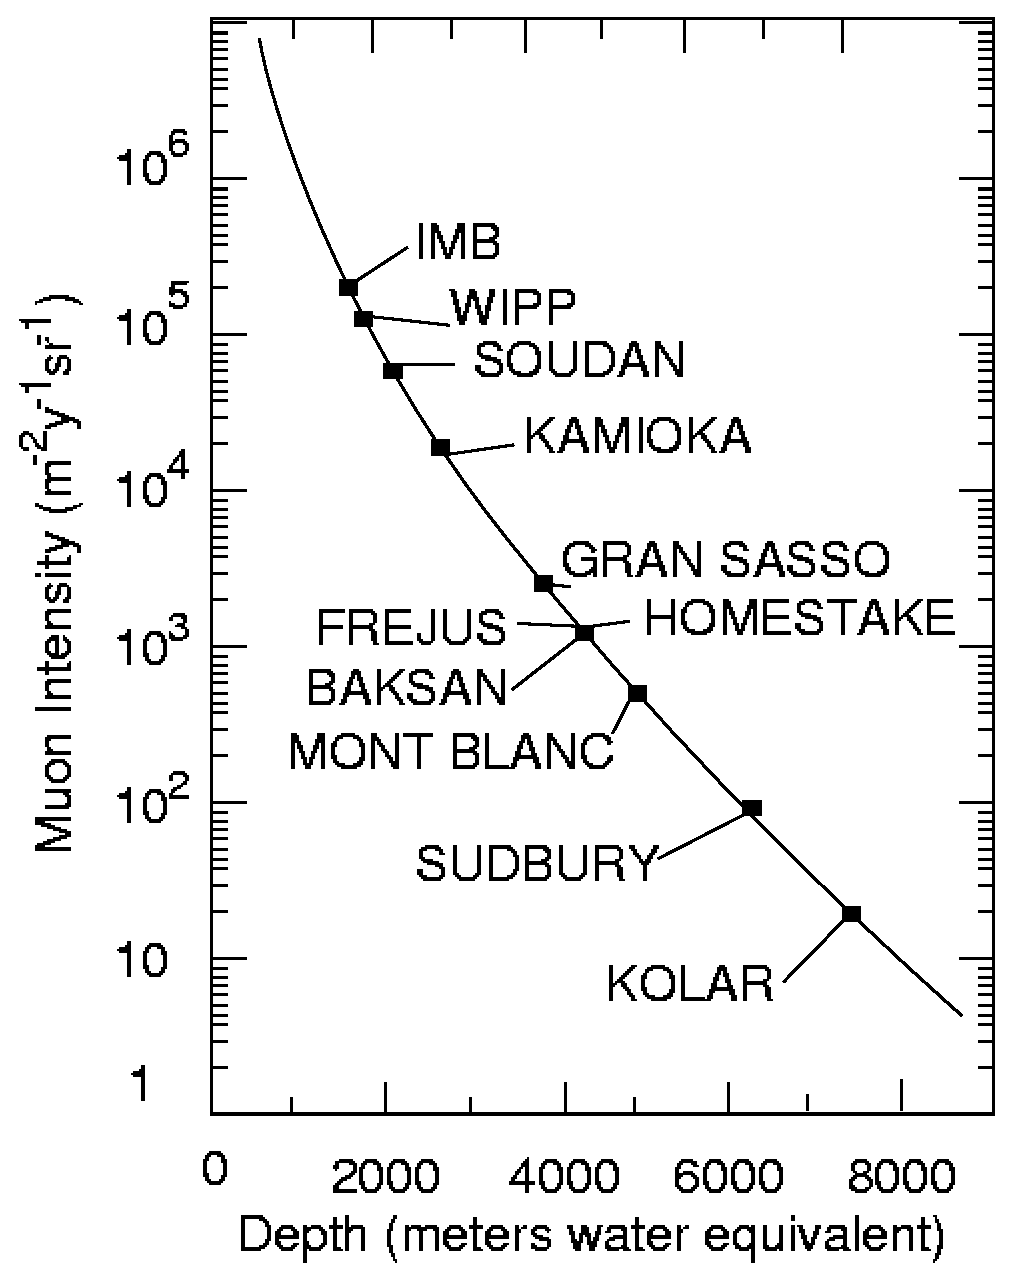
\includegraphics[keepaspectratio=true,width=\textwidth]{muonflux.eps}\\
\tiny Esch et al., NIM A 2005.
\end{column}
\end{columns}
\end{frame}

\begin{frame}
\begin{center}
\frametitle{EXO-200 TPC}
\end{center}
\vspace{1cm}
\begin{columns}[onlytextwidth]
\begin{column}{.25\textwidth}
110 kg of liquid xenon in active volume, enriched to 80.6\% in $^{136}$Xe, contained in a time projection chamber (TPC).\\[\baselineskip]
Xenon continuously circulates through purifiers outside of the cryostat.
\end{column}
\begin{column}{.75\textwidth}
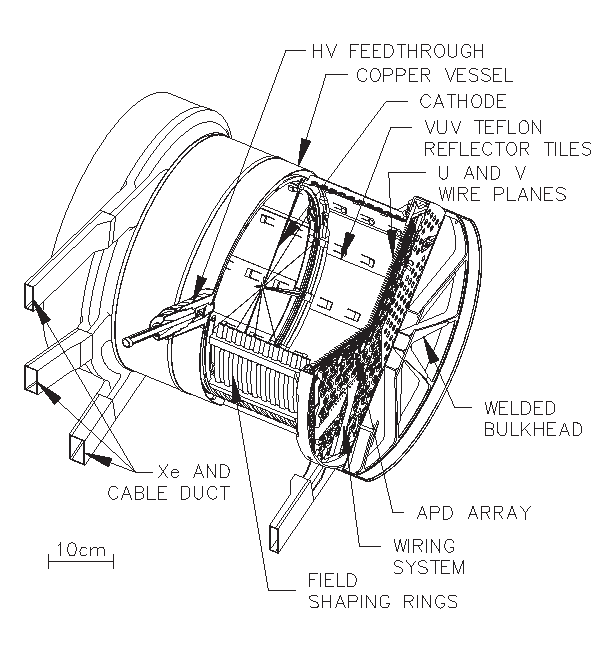
\includegraphics[keepaspectratio=true,width=\textwidth]{TPCSchematic.eps}
\end{column}
\end{columns}
\end{frame}

\begin{frame}
\begin{center}
\frametitle{EXO-200 TPC}
\end{center}
\vspace{1cm}
\begin{center}
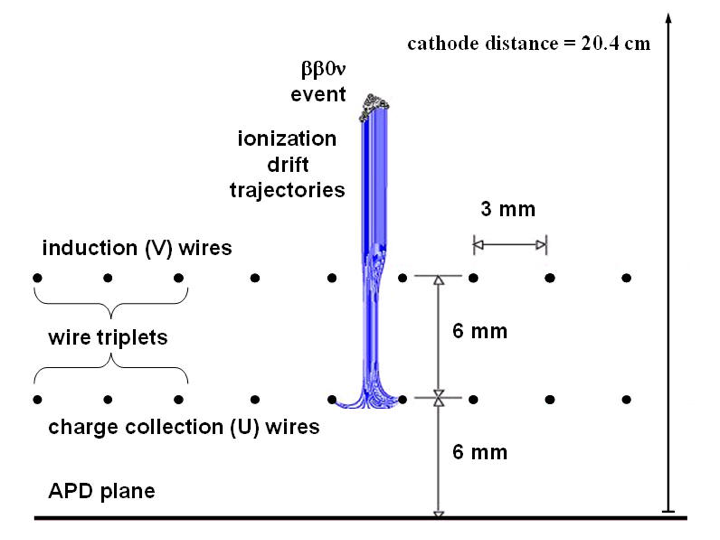
\includegraphics[keepaspectratio=true,width=.8\textwidth]{ChargeDrift2DModel.png}
\end{center}
Charge drifts under an electric field and is collected by wires on the anodes.  Light is observed by APDs behind the wires.
\end{frame}

\begin{frame}
\begin{center}
\frametitle{Energy from Ionization and Scintillation}
\end{center}
\begin{columns}
\begin{column}{.75\textwidth}
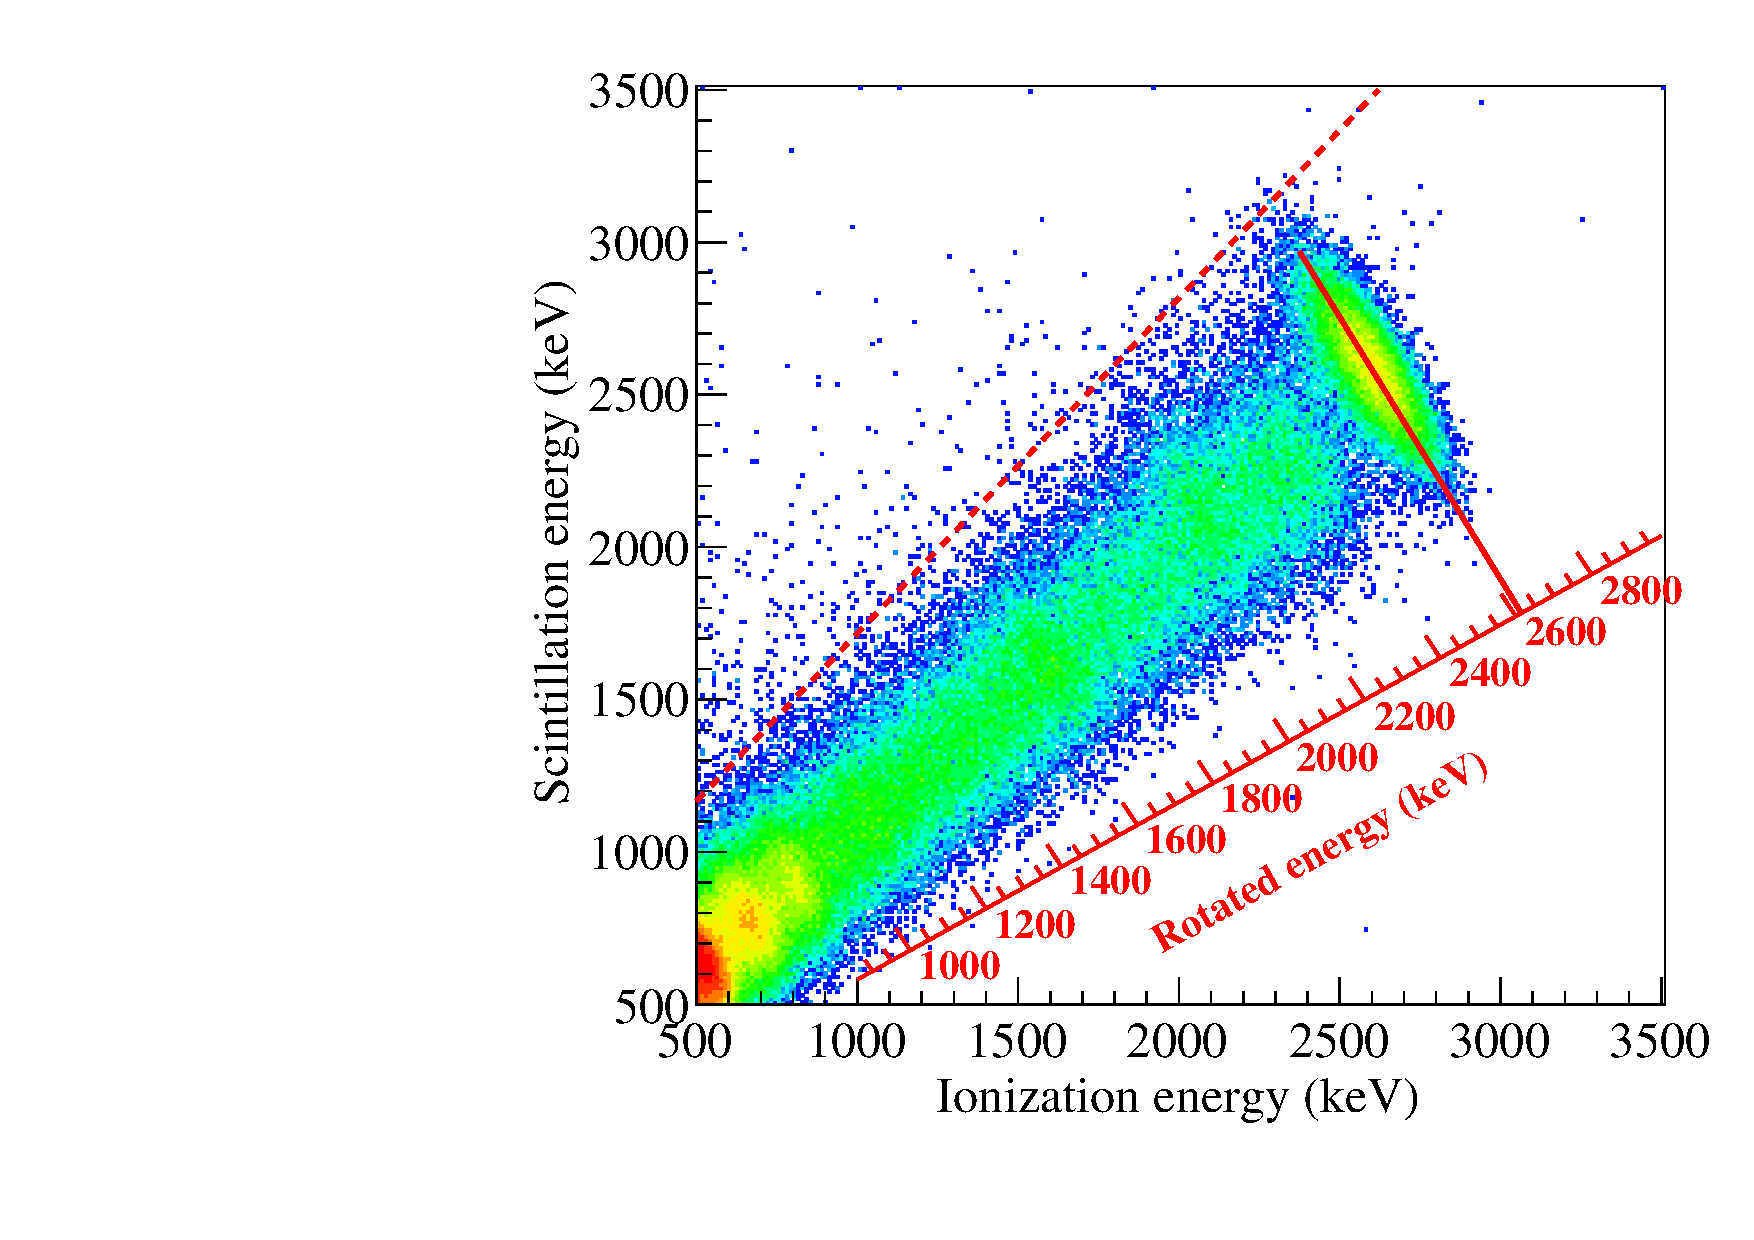
\includegraphics[keepaspectratio=true,width=\textwidth]{RotationTh2D_withCalibration.pdf}
\end{column}
\begin{column}{.25\textwidth}
Energy is independently measured from scintillation and ionization.\\[\baselineskip]

They are anticorrelated -- better energy resolution from both together than either independently.
\end{column}
\end{columns}
\end{frame}

\begin{frame}
\begin{center}
\frametitle{\hfill Primary Backgrounds:\\\hfill \textcolor{red}{$^{232}$Th}, $^{238}$U, and $^{137}$Xe}
\end{center}
\begin{columns}
\begin{column}{.6\textwidth}
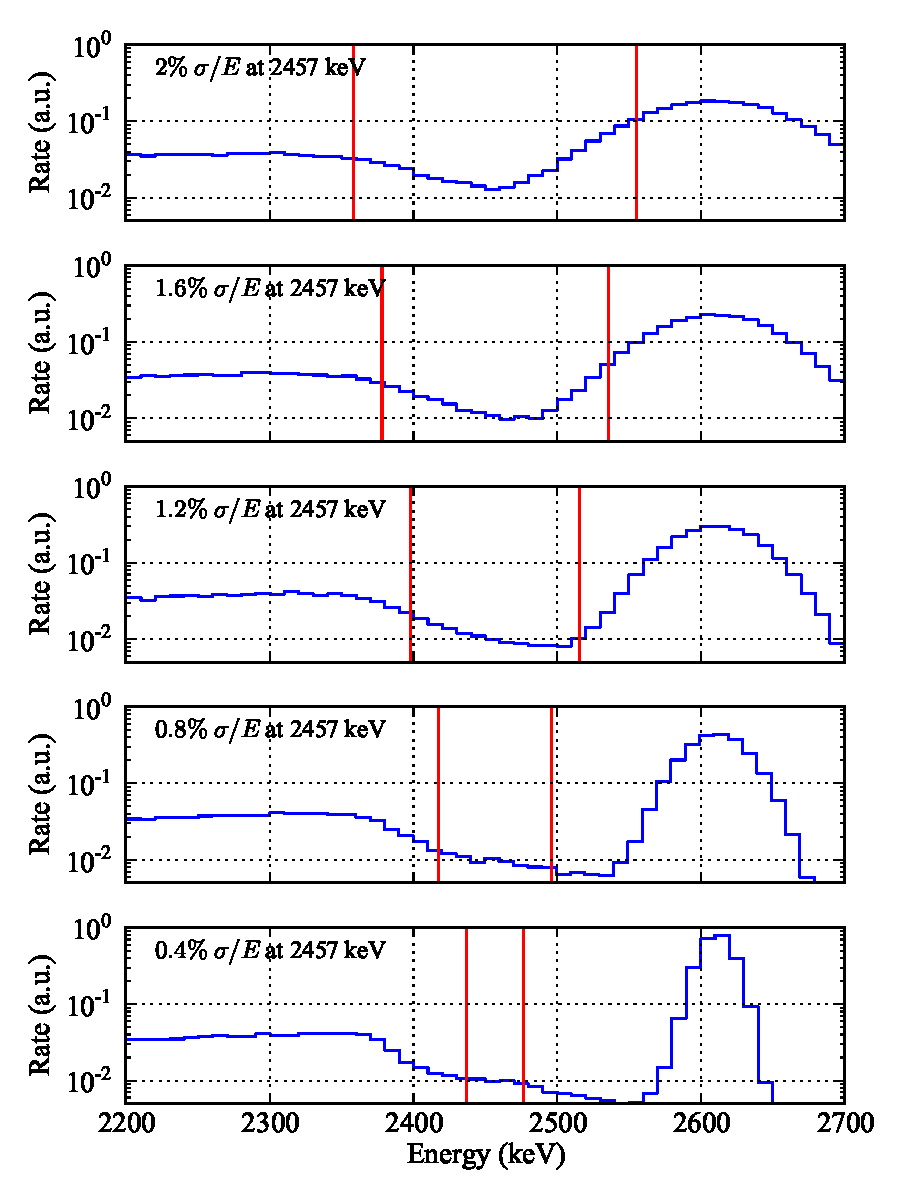
\includegraphics[keepaspectratio=true,width=\textwidth]{Th_Spectra_vs_Res.pdf}
\end{column}
\begin{column}{.4\textwidth}
Not all backgrounds are smooth.  $^{232}$Th has a gamma line at 2615 keV, so resolution reduces background sharply until 2457 and 2615 keV are well-separated around 1.2\%.\\[\baselineskip]

Beyond that, resolution for $^{232}$Th is less important (though still helpful).

\textcolor{red}{Adjust text to reflect changed ordering of slides.}
\end{column}
\end{columns}
\end{frame}

\begin{frame}
\begin{center}
\frametitle{\hfill Primary Backgrounds:\\\hfill $^{232}$Th, \textcolor{red}{$^{238}$U}, and $^{137}$Xe}
\end{center}
\begin{columns}
\begin{column}{.6\textwidth}
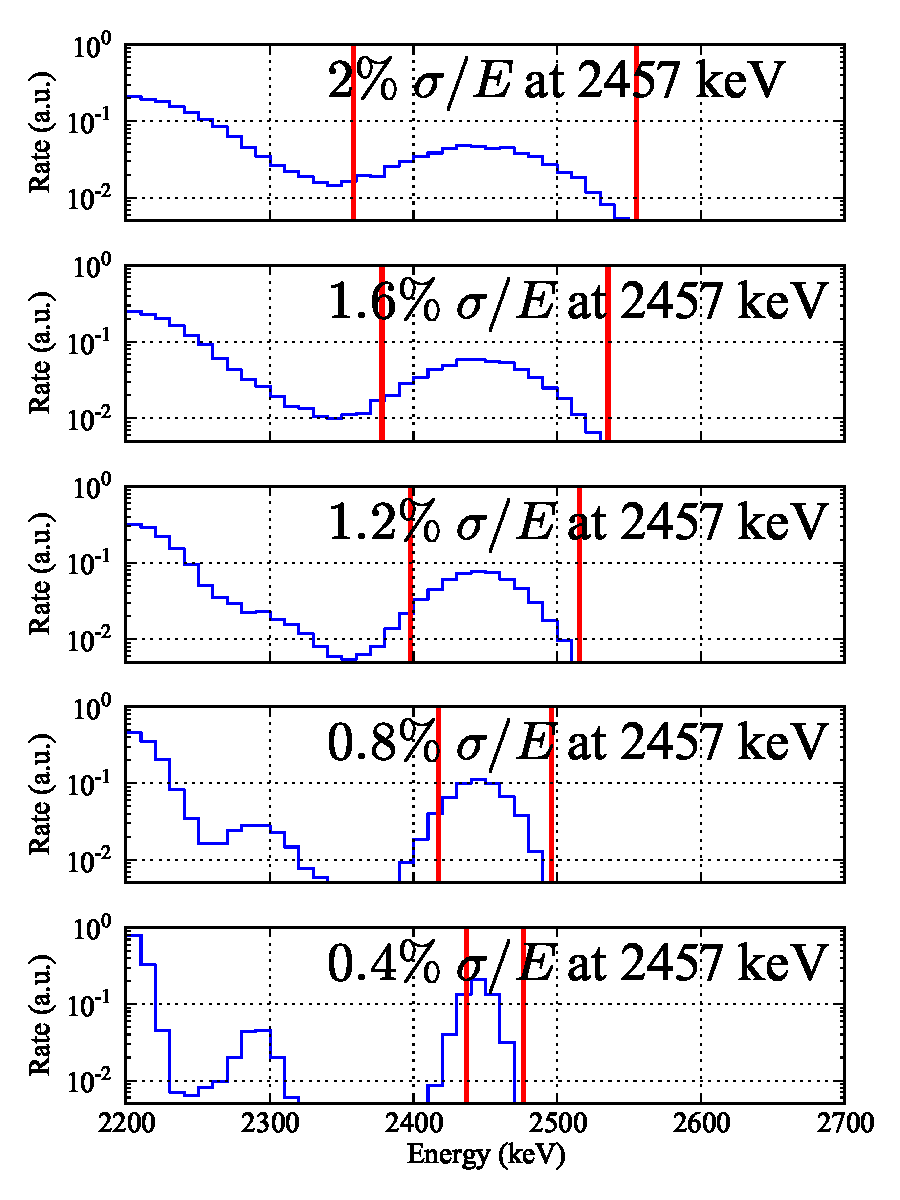
\includegraphics[keepaspectratio=true,width=\textwidth]{U_Spectra_vs_Res.pdf}
\end{column}
\begin{column}{.4\textwidth}
\vspace{0.5cm}

$^{238}$U has a 2448-keV gamma line, indistinguishable from 2457-keV $Q$-value except with extremely good resolution.\\[\baselineskip]

So, even down to 0.4\% energy resolution, most of the $^{238}$U peak at 2448 keV is still within our energy window.  $^{238}$U backgrounds aren't significantly reduced by resolution improvements.
\end{column}
\end{columns}
\end{frame}

\begin{frame}
\begin{center}
\frametitle{\hfill Primary Backgrounds:\\\hfill $^{232}$Th, $^{238}$U, and \textcolor{red}{$^{137}$Xe}}
\end{center}
\begin{columns}
\begin{column}{.6\textwidth}
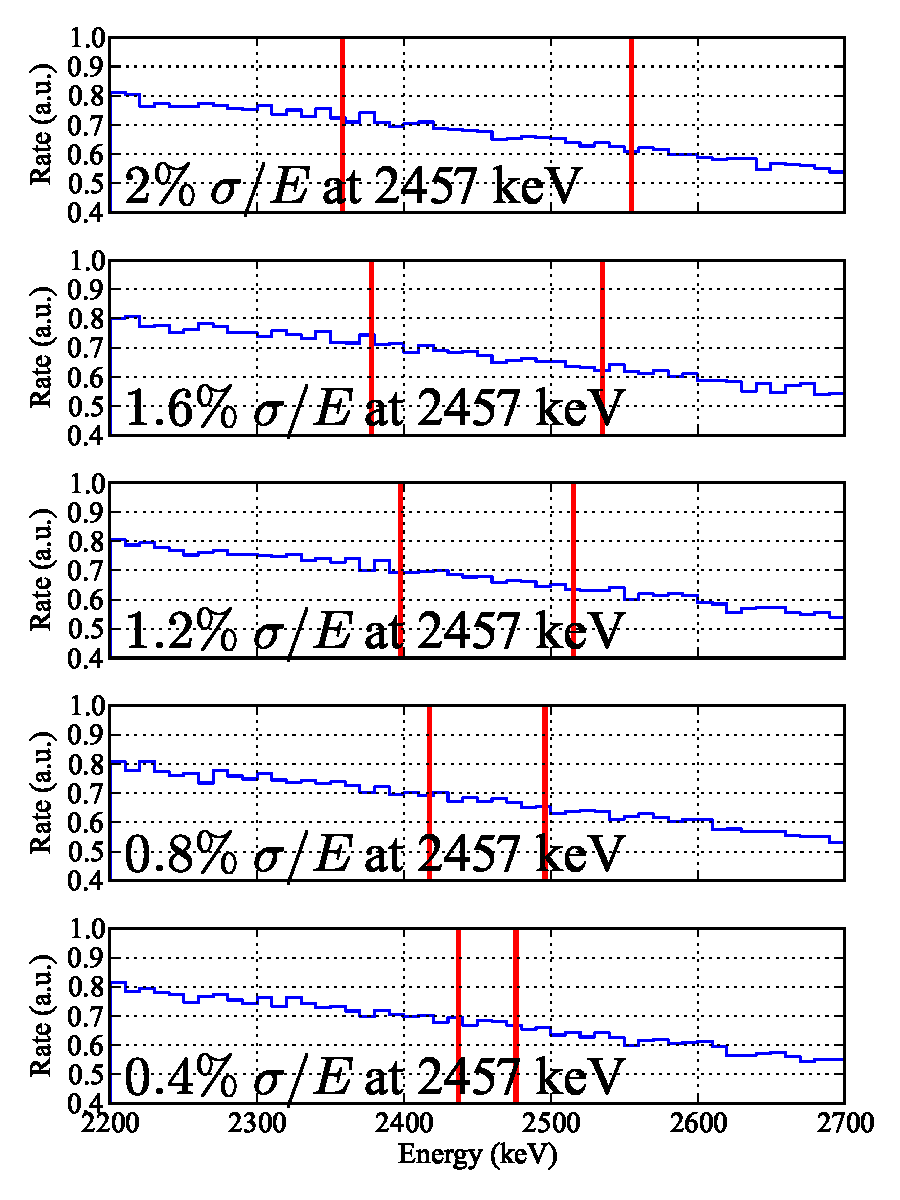
\includegraphics[keepaspectratio=true,width=\textwidth]{Xe_Spectra_vs_Res.pdf}
\end{column}
\begin{column}{.4\textwidth}
\vspace{.5cm}

Energy resolution is measured as $\sigma$/mean of a mono-energetic peak at the $Q$-value.  Typically 1.5-2\% for EXO-200.\\[\baselineskip]

Better resolution gives a sharper $\beta\beta 0\nu$ peak, so less background in that energy window.\\[\baselineskip]

$^{137}$Xe spectrum is smooth around $Q$-value; background proportional to energy resolution.
\end{column}
\end{columns}
\end{frame}

\begin{frame}
\begin{center}
\frametitle{Backgrounds vs. Resolution}
\end{center}
\vspace{1cm}
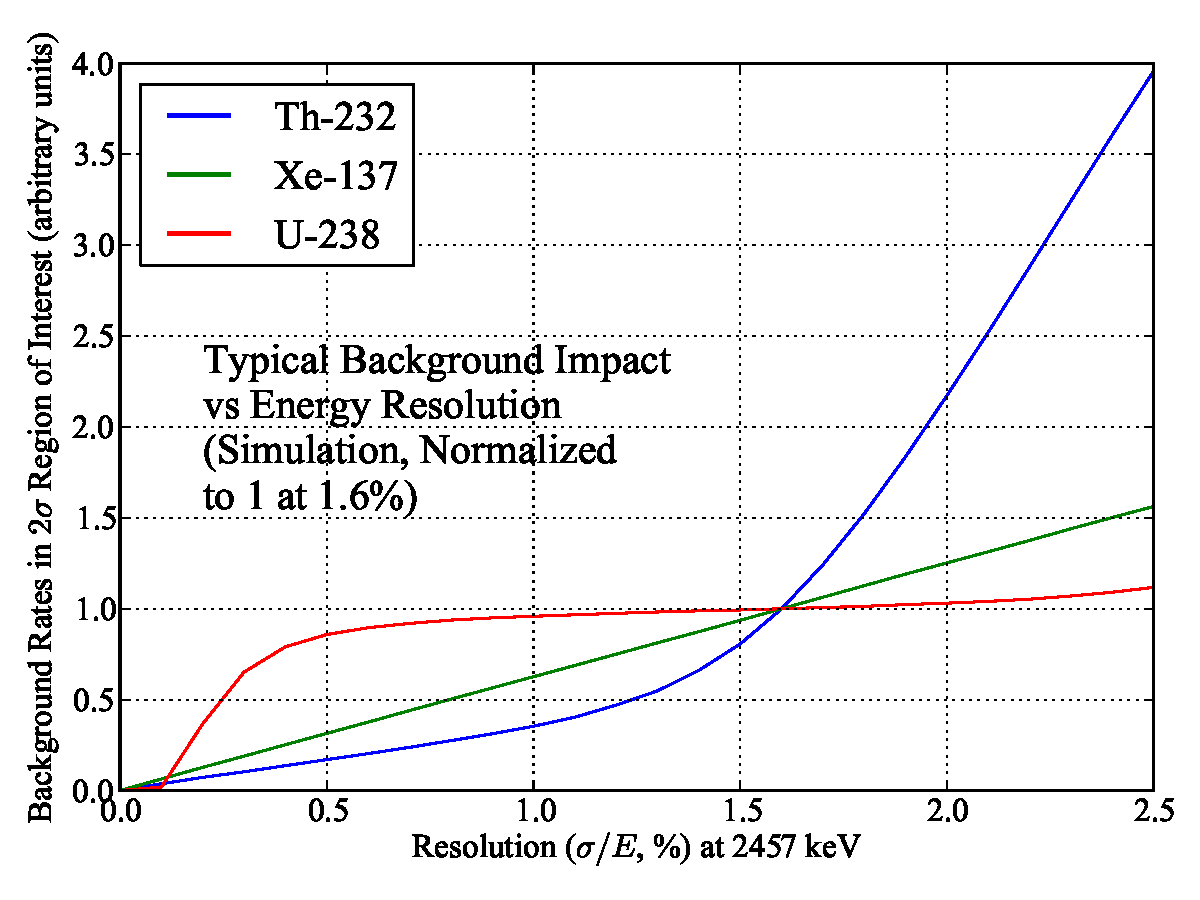
\includegraphics[keepaspectratio=true,width=\textwidth]{BackgroundsVsRes.pdf}
\end{frame}

\begin{frame}
\begin{center}
\frametitle{Time Variation of Resolution}
\end{center}
\vspace{1cm}
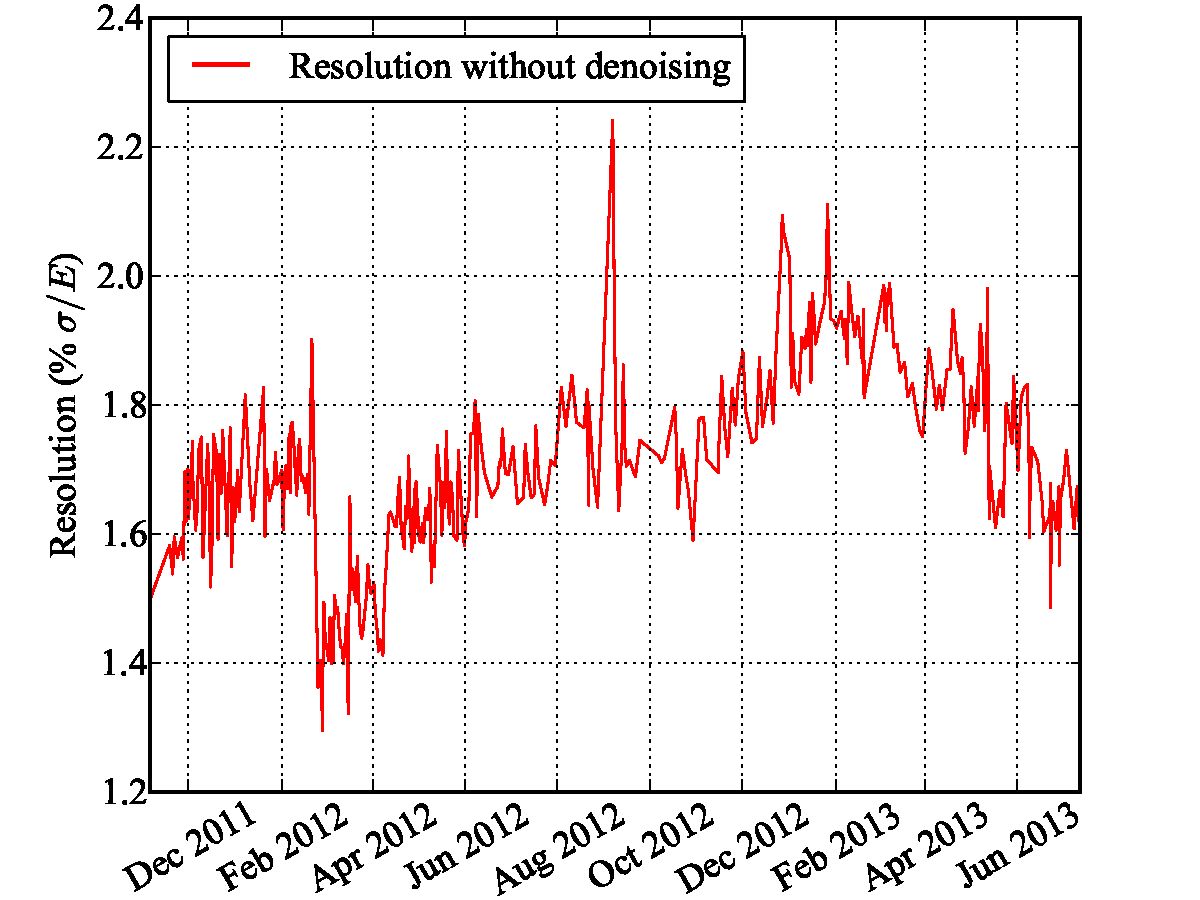
\includegraphics[keepaspectratio=true,width=\textwidth]{ResolutionNoNoiseComparison.pdf}
\end{frame}

\begin{frame}
\begin{center}
\frametitle{Time Variation of Resolution}
\end{center}
\vspace{1cm}
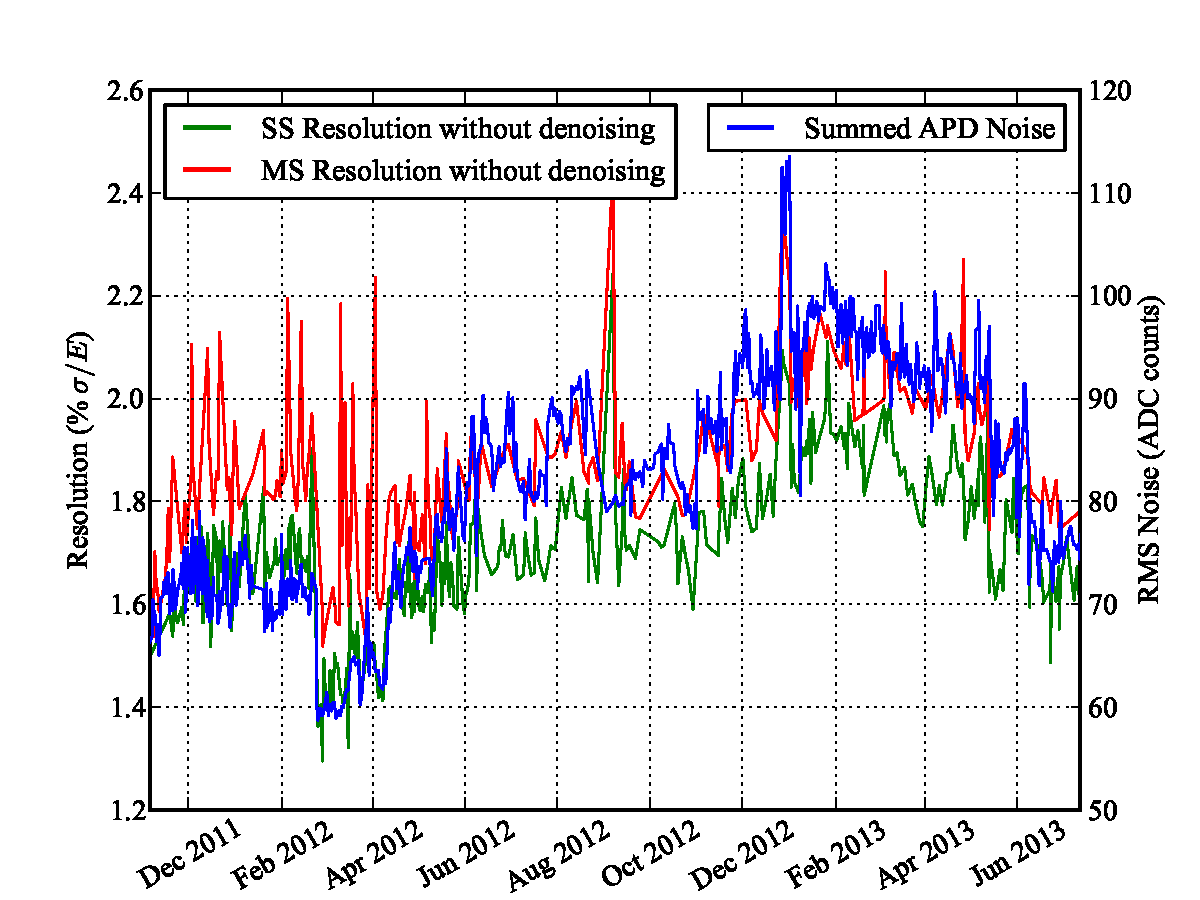
\includegraphics[keepaspectratio=true,width=\textwidth]{ResolutionAPDNoiseComparison.pdf}
\end{frame}

% Hard to see (bad contrast).
%\begin{frame}
%\begin{center}
%\frametitle{APD Noise is Correlated across Channels}
%\end{center}
%\vspace{1cm}
%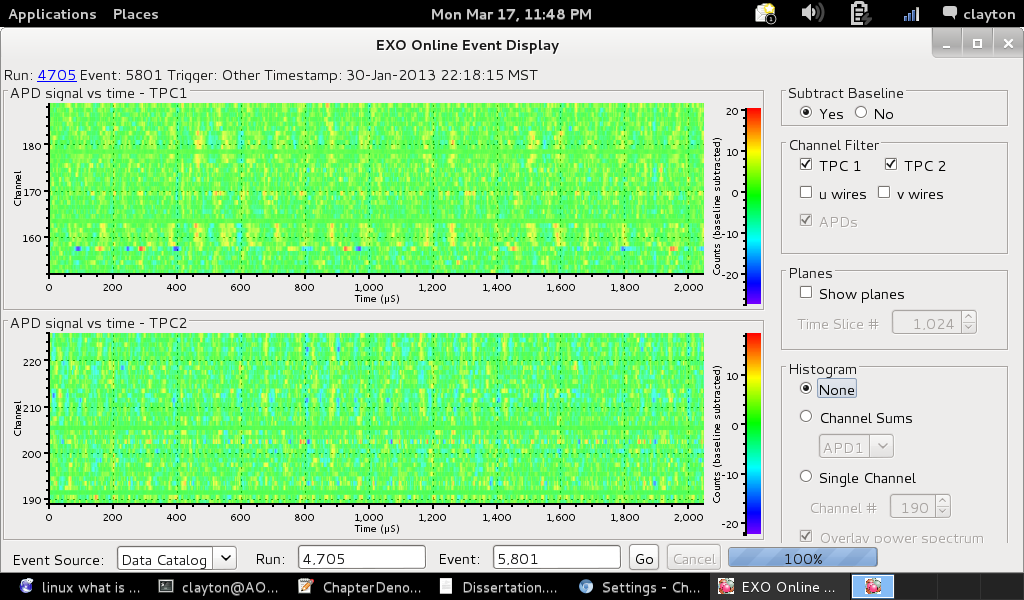
\includegraphics[keepaspectratio=true,width=\textwidth,clip=true,trim=1mm 21mm 91mm 24mm]{Run4705Ev5801_noiseEventDisplay.png}\\
%\uncover<2>{Correlated noise $\Rightarrow$ offline denoising of some sort should work!}
%\end{frame}

\begin{frame}
\begin{center}
\frametitle{APD Noise is Correlated across Channels}
\end{center}
\vspace{1cm}
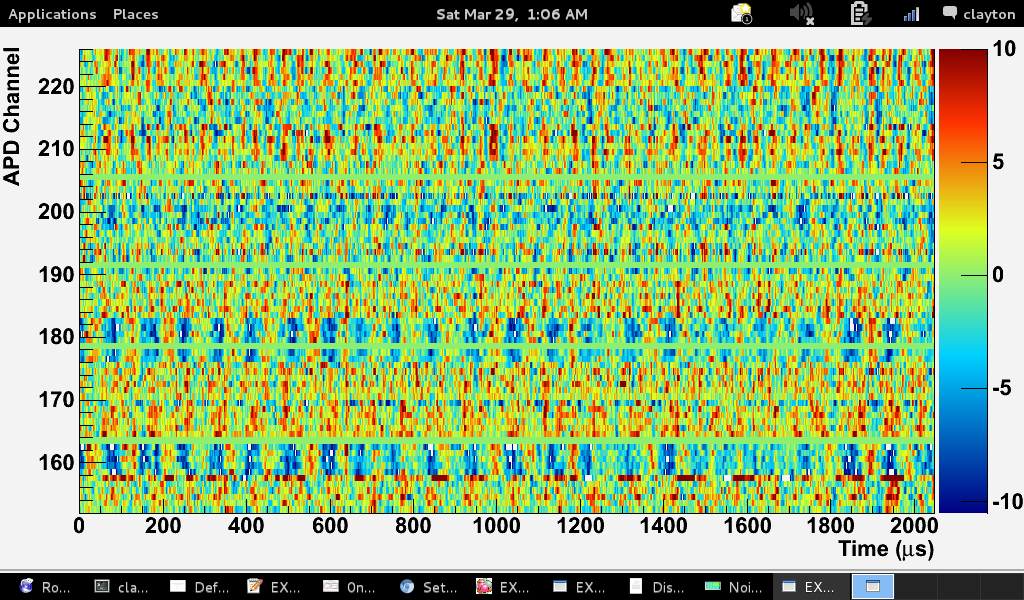
\includegraphics[keepaspectratio=true,width=\textwidth,clip=true,trim=0mm 12mm 0mm 10mm]{Run4705Ev2_noiseEventDisplay.png}\\
\uncover<2>{Correlated noise $\Rightarrow$ offline denoising of some sort should work!}
\end{frame}

\section{Denoising}

\begin{frame}
\begin{center}
\frametitle{Types of Noise}
\end{center}
Three types of noise in the scintillation measurements:
\begin{itemize}[leftmargin=*]
\item Electronic noise.\hfill\uncover<2,4->{$\leftarrow$ Additive; use fewer channels.}
\item Photon fluctuations.\hfill\uncover<3->{$\leftarrow$ Poissonian; use more channels.}
\item Gain fluctuations.\hfill\uncover<3->{$\leftarrow$ Poissonian; use more channels.}
\end{itemize}
A ``denoising'' algorithm should minimize all three.\\[\baselineskip]

\uncover<4->{Most denoising algorithms transform an input waveform to an output waveform, with pulses amplified and additive noise reduced.\\[\baselineskip]

Here we're trying to reduce the impact of noise which is correlated with pulses.  That means traditional denoising won't accomplish what we need.\\[\baselineskip]

So, ``denoising'' for us means producing a noise-tolerant estimate of the scintillation energy.}
\end{frame}

\begin{frame}
\begin{center}
\frametitle{Types of Denoising}
\end{center}
\vspace{1cm}
There are also three approaches to reducing the impact of noise:
\begin{itemize}
\item<1,2> Frequency weighting.
\item<1,3> Channel weighting.
\item<1,4> Exploit noise correlations.
\end{itemize}
\begin{center}
\parbox [t][60mm]{\textwidth}{ % To avoid jitter from changing vertical spacing.
\only<2>{
\vspace{-0.5cm}\hfill Noise and pulse power spectra.\\
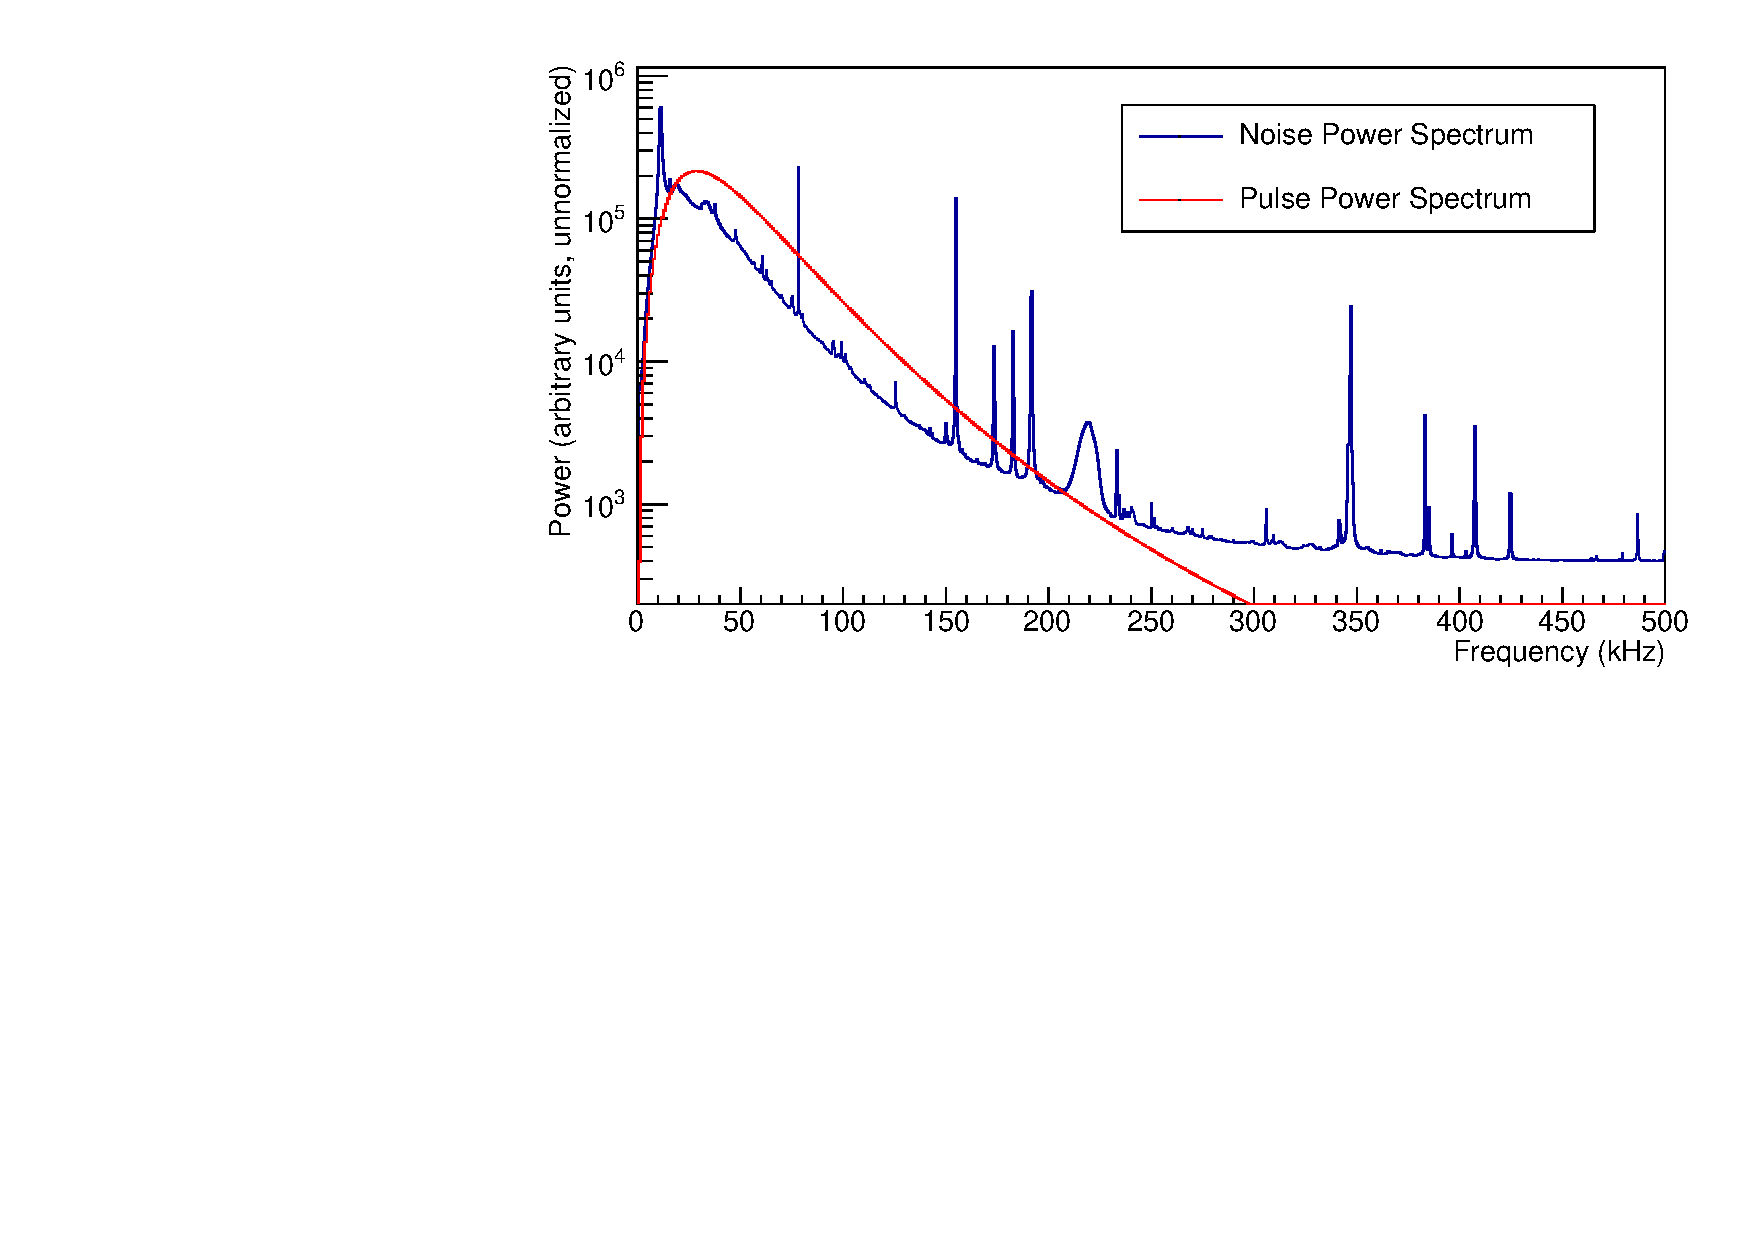
\includegraphics[keepaspectratio=true,width=\textwidth]{NoisePowerSpectrum.pdf}} % Channel 152 noise
\only<3>{
\vspace{-0.5cm}\hfill APD pulse magnitudes.\\[0.5\baselineskip]
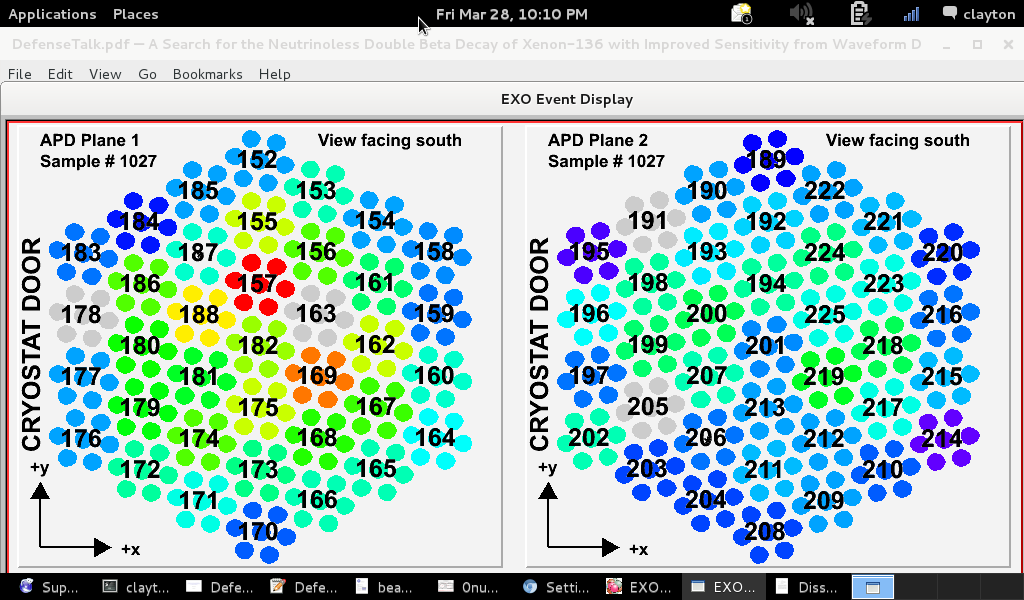
\includegraphics[keepaspectratio=true,width=\textwidth,clip=true,trim=5mm 10mm 5mm 44mm]{APD_Planes.png}} % Run 4705 event 5799
\only<4>{
\vspace{-0.5cm}\hfill Noise correlations at 78.6 kHz.\\
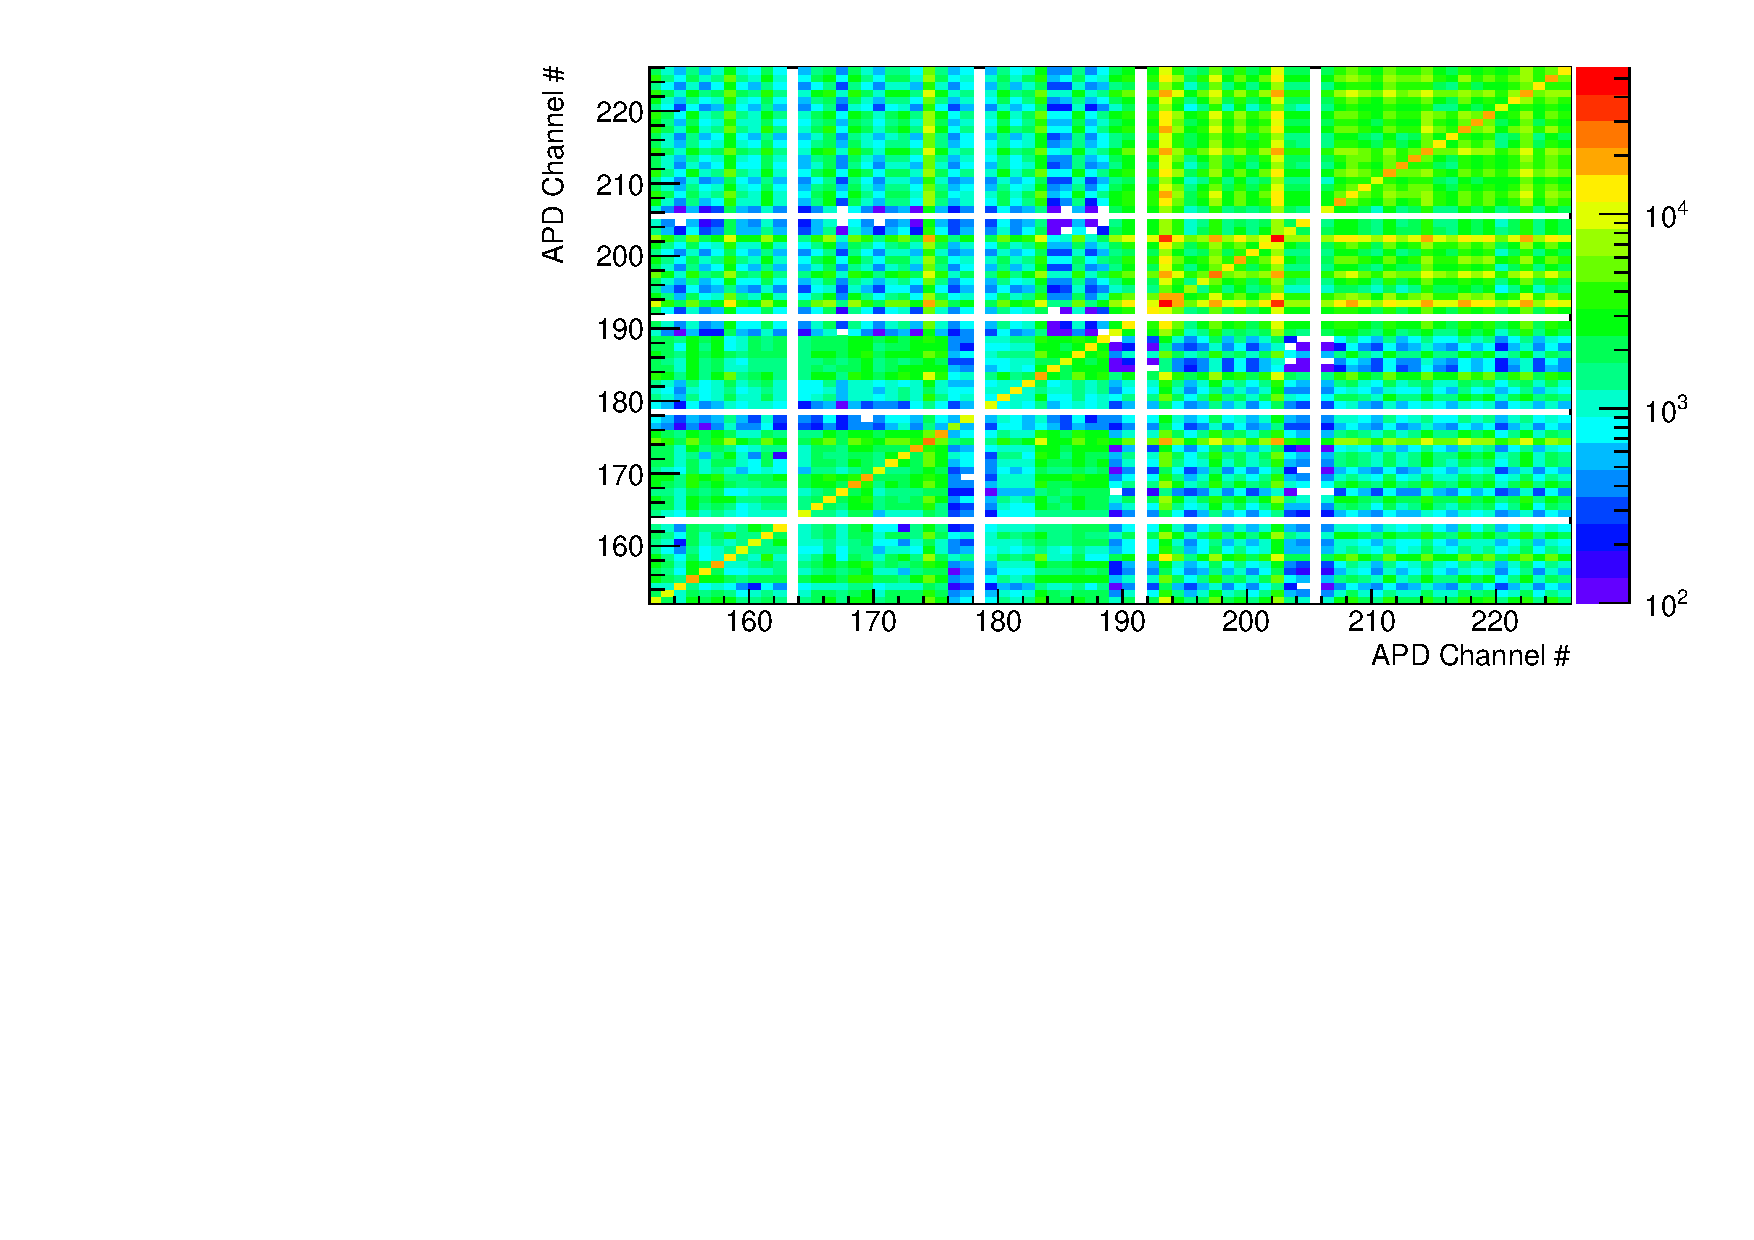
\includegraphics[keepaspectratio=true,width=\textwidth]{NoiseHeatPlot_161.pdf}} %Corresponding to frequency 78.6 kHz (f=161).
}\end{center}
\end{frame}

\begin{frame}
\begin{center}
\frametitle{Waveform Model}
\end{center}
\vspace{0.5cm}
When there is one energy deposit in the xenon, the APD waveform $X_i[f]$ (in frequency space) on channel $i$ can be modeled:
\[X_i[f] = M_i Y_i[f] + N_i[f]\text{, where:}\]
\begin{itemize}
\item $Y_i[f]$ is the unit-magnitude template pulse for channel $i$.
\item $M_i$ is the magnitude of the pulse observed on channel $i$, including the scintillation energy and Poisson fluctuations in photon statistics and gain.
\item $N_i[f]$ is the additive (electronic) noise on channel $i$.\\[\baselineskip]
\end{itemize}

To complete our model, we need to understand the distributions of the random variables:
\begin{itemize}
\item How $M_i$ depends on the unknown energy $E$.
\item How magnitudes $M_i$ and $M_j$ are correlated.
\item How electronic noise $N_i[f]$ and $N_j[f]$ are correlated.
\end{itemize}
\end{frame}

\begin{frame}
\begin{center}
\frametitle{Electronic Noise}
\end{center}
To measure the electronic (additive) noise, we need waveforms with no pulse.

Fortunately, EXO-200 is a low-background detector: most of the time all it measures is noise.\\[\baselineskip]

So, this is fairly easy: use our noise data to measure all of the pairwise noise correlations.

Explicitly, we measure:\\
\begin{center}
$\left<N_i^R[f]N_j^R[f]\right>$, $\left<N_i^R[f]N_j^I[f]\right>$, and $\left<N_i^I[f]N_j^I[f]\right>$,\\
\end{center}
where $N_i^R[f]$ and $N_i^I[f]$ are the real and imaginary parts of $N_i[f]$.
\end{frame}

\begin{frame}
\begin{center}
\frametitle{Electronic Noise}
\end{center}
\vspace{1cm}
Main detail: the electronic noise changes over time (mostly in discontinuous steps).
\begin{center}
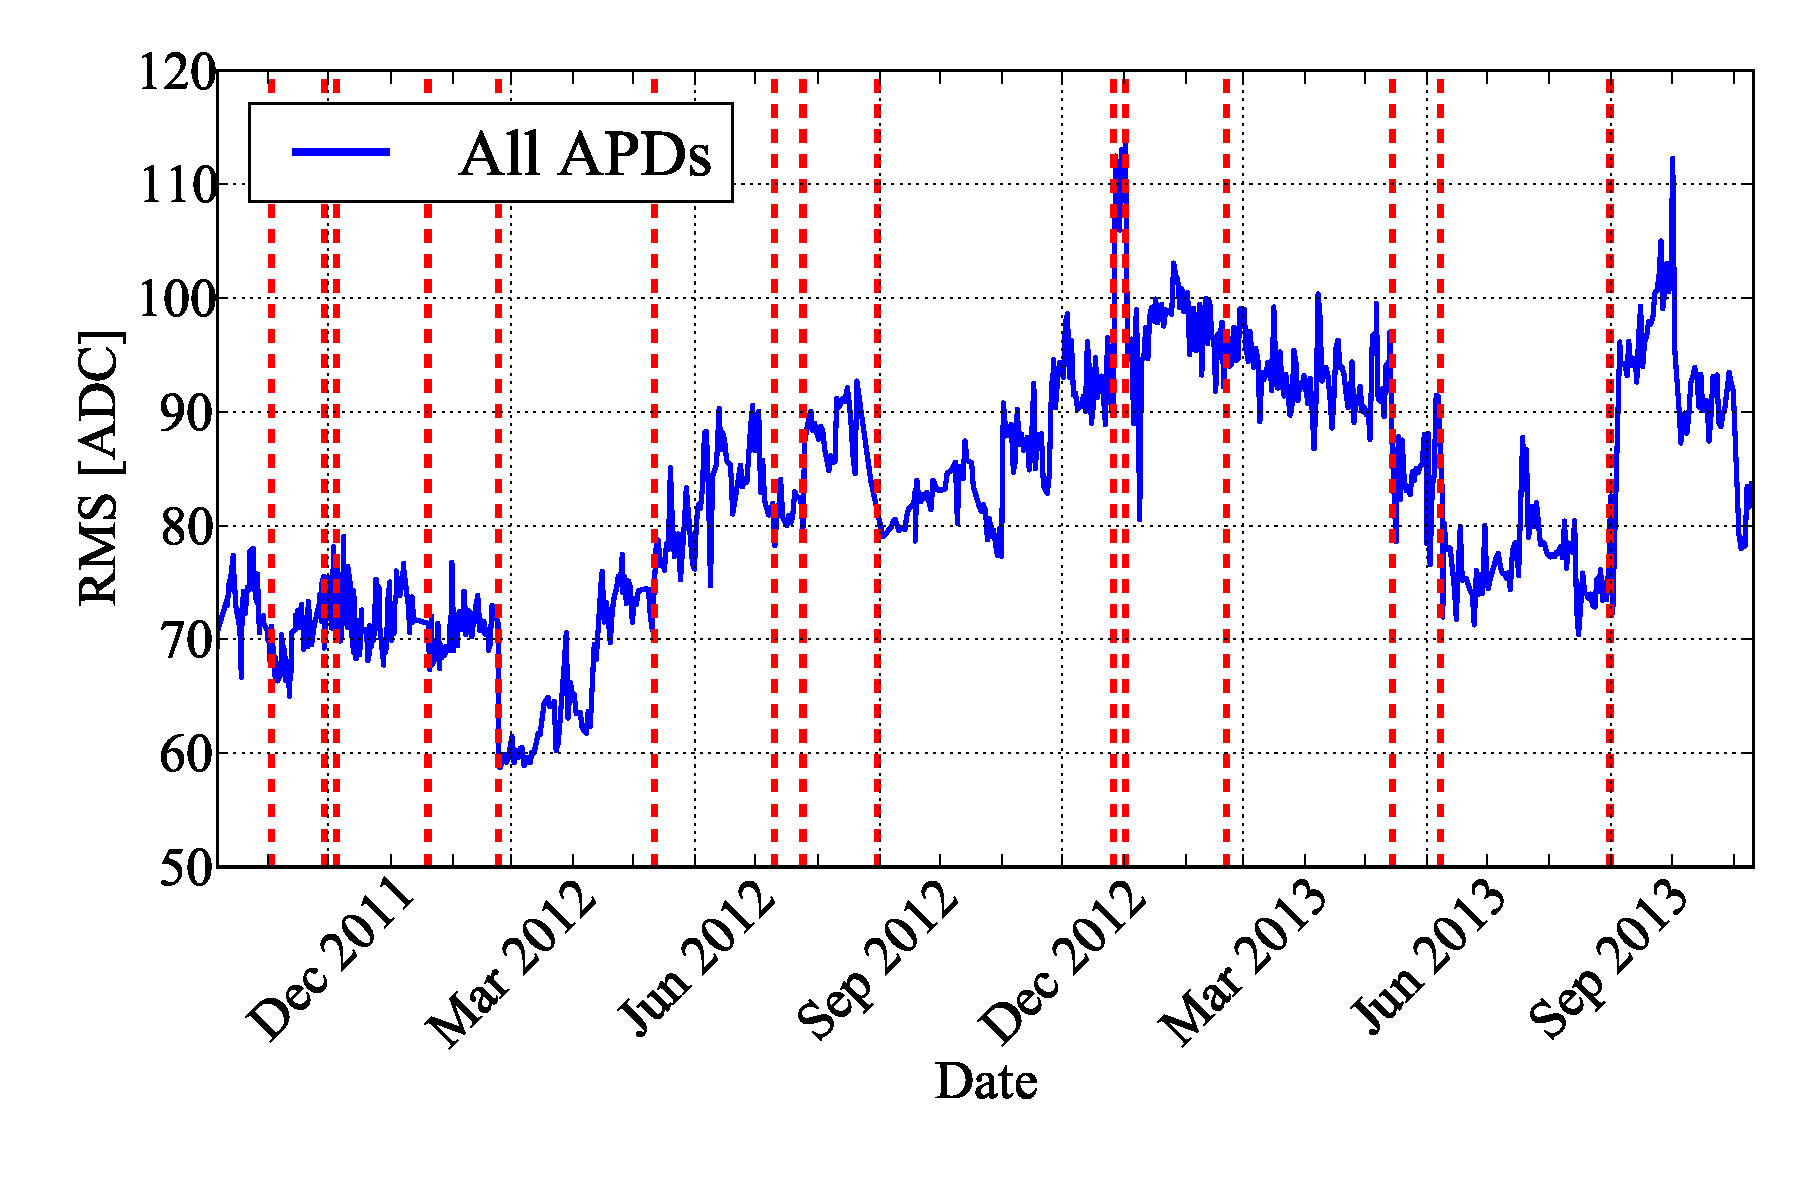
\includegraphics[keepaspectratio=true,width=\textwidth,clip=true,trim=5mm 0mm 0mm 0mm]{APDNoiseVsActions_sumall.pdf}
\end{center}
\end{frame}

\begin{frame}
\begin{center}
\frametitle{Lightmaps}
\end{center}
\vspace{1cm}
The expected pulse height $M_i$ on a channel $i$ from a deposit at position $\vec{x}$ and time $t$ is described by a lightmap $L_i(\vec{x},t)$:
\[\left<M_i\right> = L_i(\vec{x},t)E.\]
\begin{center}
\parbox [t][70mm]{\textwidth}{ % To avoid jitter from changing vertical spacing.
\only<1>{To measure $L_i(\vec{x},t)$, we need a known-energy deposit for all position and time bins.  But we don't have that much data: calibration sources give us good statistics, but aren't near every position.
\begin{center}
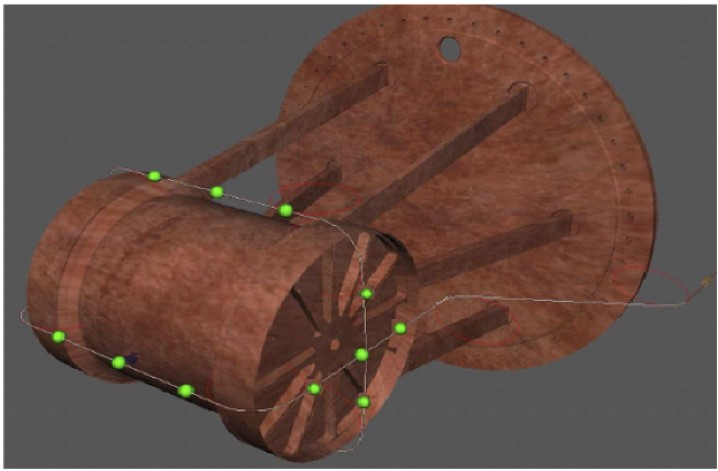
\includegraphics[keepaspectratio=true,width=.8\textwidth,clip=true,trim=0mm 0mm 0mm 50mm]{calibration_tube.jpg}
\end{center}}
\only<2>{To reduce the amount of statistics needed, we make an approximation that $L_i(\vec{x},t)$ is separable into spatial and temporal components:
\[L_i(\vec{x},t) = R_i(\vec{x})S_i(t).\]
So, rather than needing one known-energy deposit per position per time, we need one per position during the whole history of EXO-200.

(We do this assuming that APD gain varies over time, but light collection does not, and gain does not depend on the position of the deposit.)}
}\end{center}
\end{frame}

\begin{frame}
\begin{center}
\frametitle{Lightmaps}
\end{center}
\vspace{1cm}
With this simpler form for the lightmap, we can measure $R_i(\vec{x})$ and $S_i(t)$ by combining all thorium source calibration events from the $^{208}$Tl 2615-keV gamma line.  It is a clean, well-isolated peak:
\begin{center}
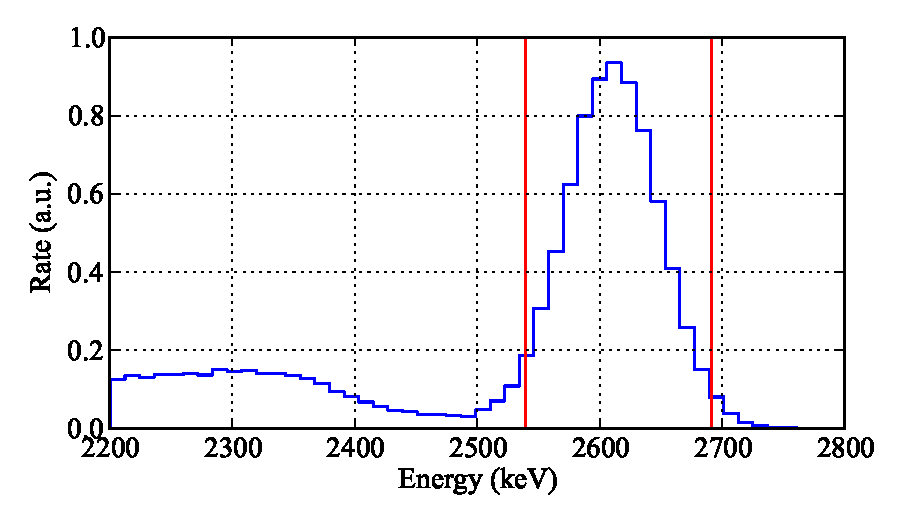
\includegraphics[keepaspectratio=true,width=\textwidth]{Th_lightmap_cuts.pdf}
\end{center}
\end{frame}

\begin{frame}
\begin{center}
\frametitle{Lightmaps: $R_i(\vec{x})$}
\end{center}
\begin{center}
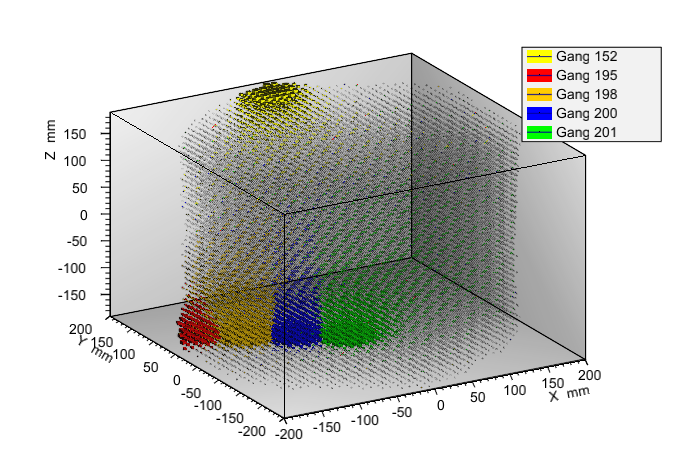
\includegraphics[keepaspectratio=true,width=\textwidth,clip=true,trim=15mm 10mm 10mm 10mm]{Lightmap_viz_zoom.png}
\end{center}
\end{frame}

\begin{frame}
\begin{center}
\frametitle{Lightmaps: $S_i(t)$ for $i = 152$}
\end{center}
\vspace{0.5cm}
\begin{center}
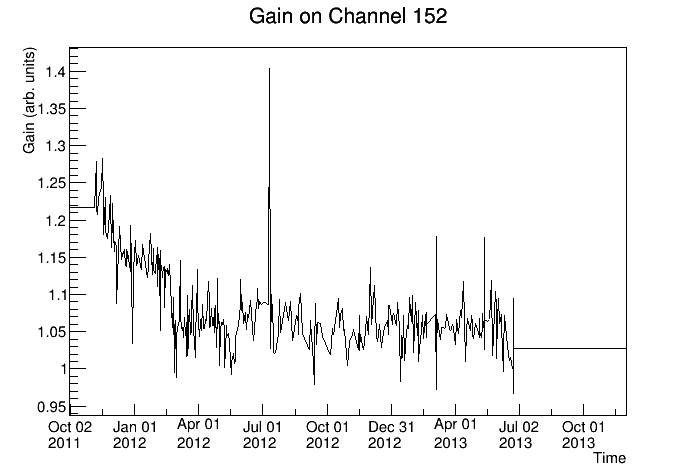
\includegraphics[keepaspectratio=true,width=\textwidth,clip=true,trim=5mm 0mm 20mm 15mm]{gainfunc_152.png}
\end{center}
\end{frame}

\begin{frame}
\newmdenv[topline=false,userdefinedwidth=2cm]{PhotonBoxStyle}
\begin{center}
\frametitle{Light Collection Noise}
\end{center}
\vspace{1cm}
The expected pulse height $M_i$ on a channel $i$ from a deposit at position $\vec{x}$ and time $t$ is described by a lightmap $L_i(\vec{x},t)$:
\[\left<M_i\right> = L_i(\vec{x},t)E.\]
What about covariances of $M_i$?\\[\baselineskip]

\parbox [t][60mm]{\textwidth}{ % To avoid jitter from changing vertical spacing.
\only<1>{
Photon collection by the APDs has a multinomial distribution:\\[-1.5\baselineskip]
\begin{framed}
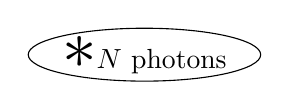
\begin{tikzpicture}
\node[draw,shape=ellipse,inner sep=0ex]{{\Huge $\ast$}$N$ photons};
\end{tikzpicture}

\hfill With photon collection $\left<P_i\right> = N\cdot f_i$,

\hfill covariances are $cov(P_i,P_j) = N \cdot \left(f_i \delta_{ij} - f_i f_j\right)$.

\begin{center}
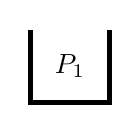
\begin{tikzpicture}
\node[draw,shape=PhotonBin,inner sep=2ex]{$P_1$};
\end{tikzpicture}
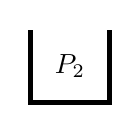
\begin{tikzpicture}
\node[draw,shape=PhotonBin,inner sep=2ex]{$P_2$};
\end{tikzpicture}
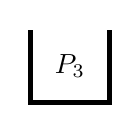
\begin{tikzpicture}
\node[draw,shape=PhotonBin,inner sep=2ex]{$P_3$};
\end{tikzpicture}
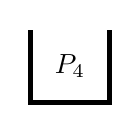
\begin{tikzpicture}
\node[draw,shape=PhotonBin,inner sep=2ex]{$P_4$};
\end{tikzpicture}
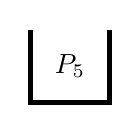
\begin{tikzpicture}
\node[draw,shape=PhotonBin,inner sep=2ex]{$P_5$};
\end{tikzpicture}
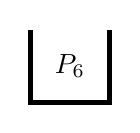
\begin{tikzpicture}
\node[draw,shape=PhotonBin,inner sep=2ex]{$P_6$};
\end{tikzpicture}
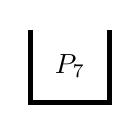
\begin{tikzpicture}
\node[draw,shape=PhotonBin,inner sep=2ex]{$P_7$};
\end{tikzpicture}
\end{center}
\end{framed}
\vspace{-1.5cm}
\begin{center}
Photons randomly deposit on APDs (or are not observed).
\end{center}
}
\only<2>{
\textcolor{red}{Show a simplified picture of an APD as:
\begin{itemize}
\item A surface where photoelectrons are produced (quantum efficiency).
\item A volume where gain is applied (gain fluctuations).
\end{itemize}
}}}
\end{frame}

\begin{frame}
\begin{center}
\frametitle{Denoising: An Optimization Problem}
\end{center}
So, the waveforms $X_i[f]$ are modeled by:
\[X_i[f] = M_i Y_i[f] + N_i[f],\]
and we have full descriptions of the random variables $M_i$ and $N_i[f]$.

Linear real-valued energy estimators $\widehat{E}$ take the form:
\[\widehat{E} = \sum_{if} A_i[f] X^R_i[f] + B_i[f] X^I_i[f],\]
where $A_i[f]$ and $B_i[f]$ are parameters we can adjust.\\[0.5\baselineskip]

Problem: minimize the mean square error, $\left<\left(E-\widehat{E}\right)^2\right>$.\\[0.5\baselineskip]
Constraint:  estimator is unbiased, $\left<E-\widehat{E}\right>=0$.
\end{frame}

\begin{frame}
\begin{center}
\frametitle{Denoising: An Optimization Problem}
\end{center}
The solution is a big matrix equation
\uncover<2>{which we write in a compact way:
\[\begin{pmatrix}\mathbf{N+P}&C^{\top}\\C & 0\end{pmatrix}\begin{pmatrix}A\\\lambda\end{pmatrix} = \begin{pmatrix}0\\1\end{pmatrix}.\]

The LHS matrix is a $143,\!291 \times 143,\!291$ sparse matrix with roughly twenty million non-zero entries.\\[\baselineskip]

We need to solve this system once {\bf for each event}, and there are hundreds of millions of events.  Fortunately this is an embarassingly parallel problem, so we can just find a big computing system and do it.\\[\baselineskip]

NERSC, at LBNL, was used for this analysis; we required roughly 50,000 core-hours to do this processing.
}
\end{frame}

\section{Results}

\begin{frame}
\begin{center}
\frametitle{$^{228}$Th Source Spectrum (Before and After)}
\end{center}
\vspace{1cm}
\begin{center}
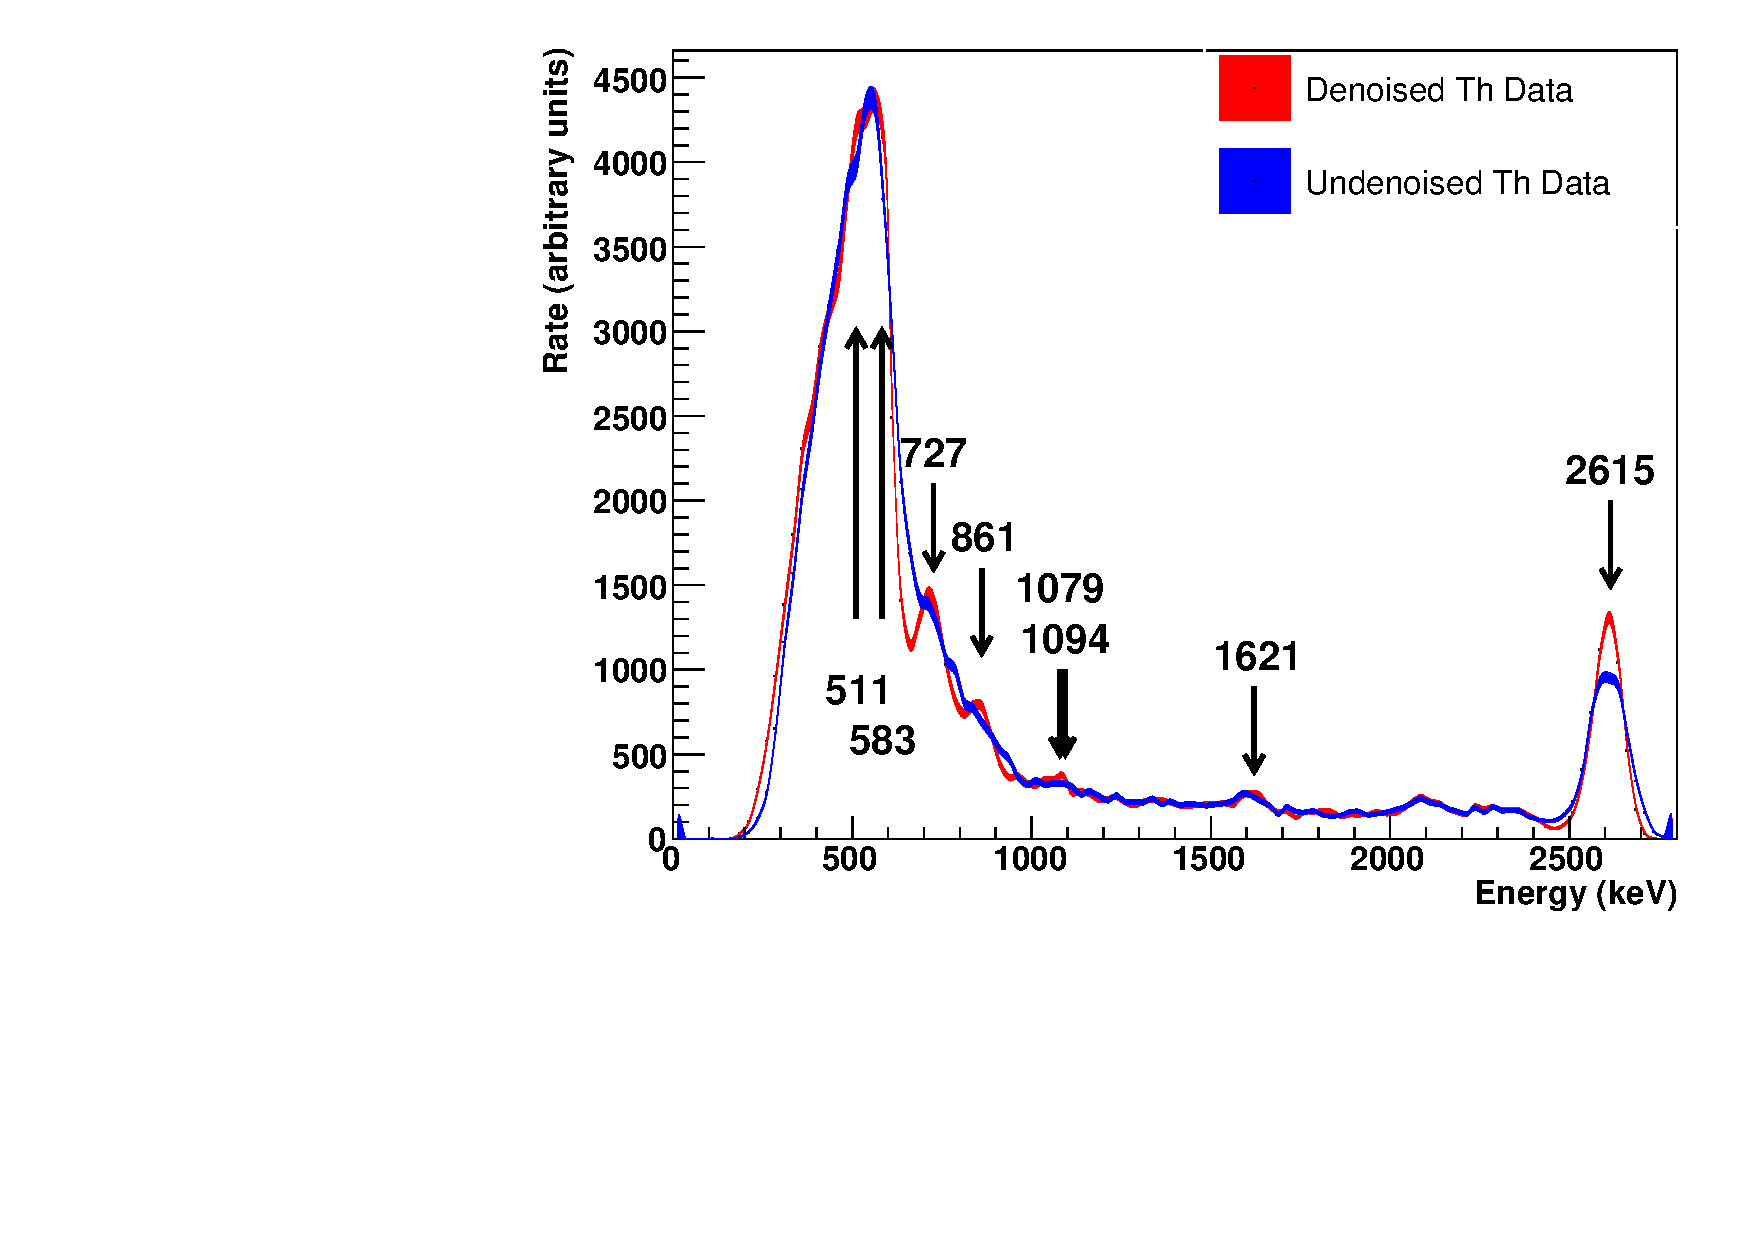
\includegraphics[keepaspectratio=true,width=\textwidth]{ThSourceSpectrumComparison.pdf}
\end{center}
\end{frame}

\begin{frame}
\begin{center}
\frametitle{$^{60}$Co Source Spectrum (Before and After)}
\end{center}
\vspace{1cm}
\begin{center}
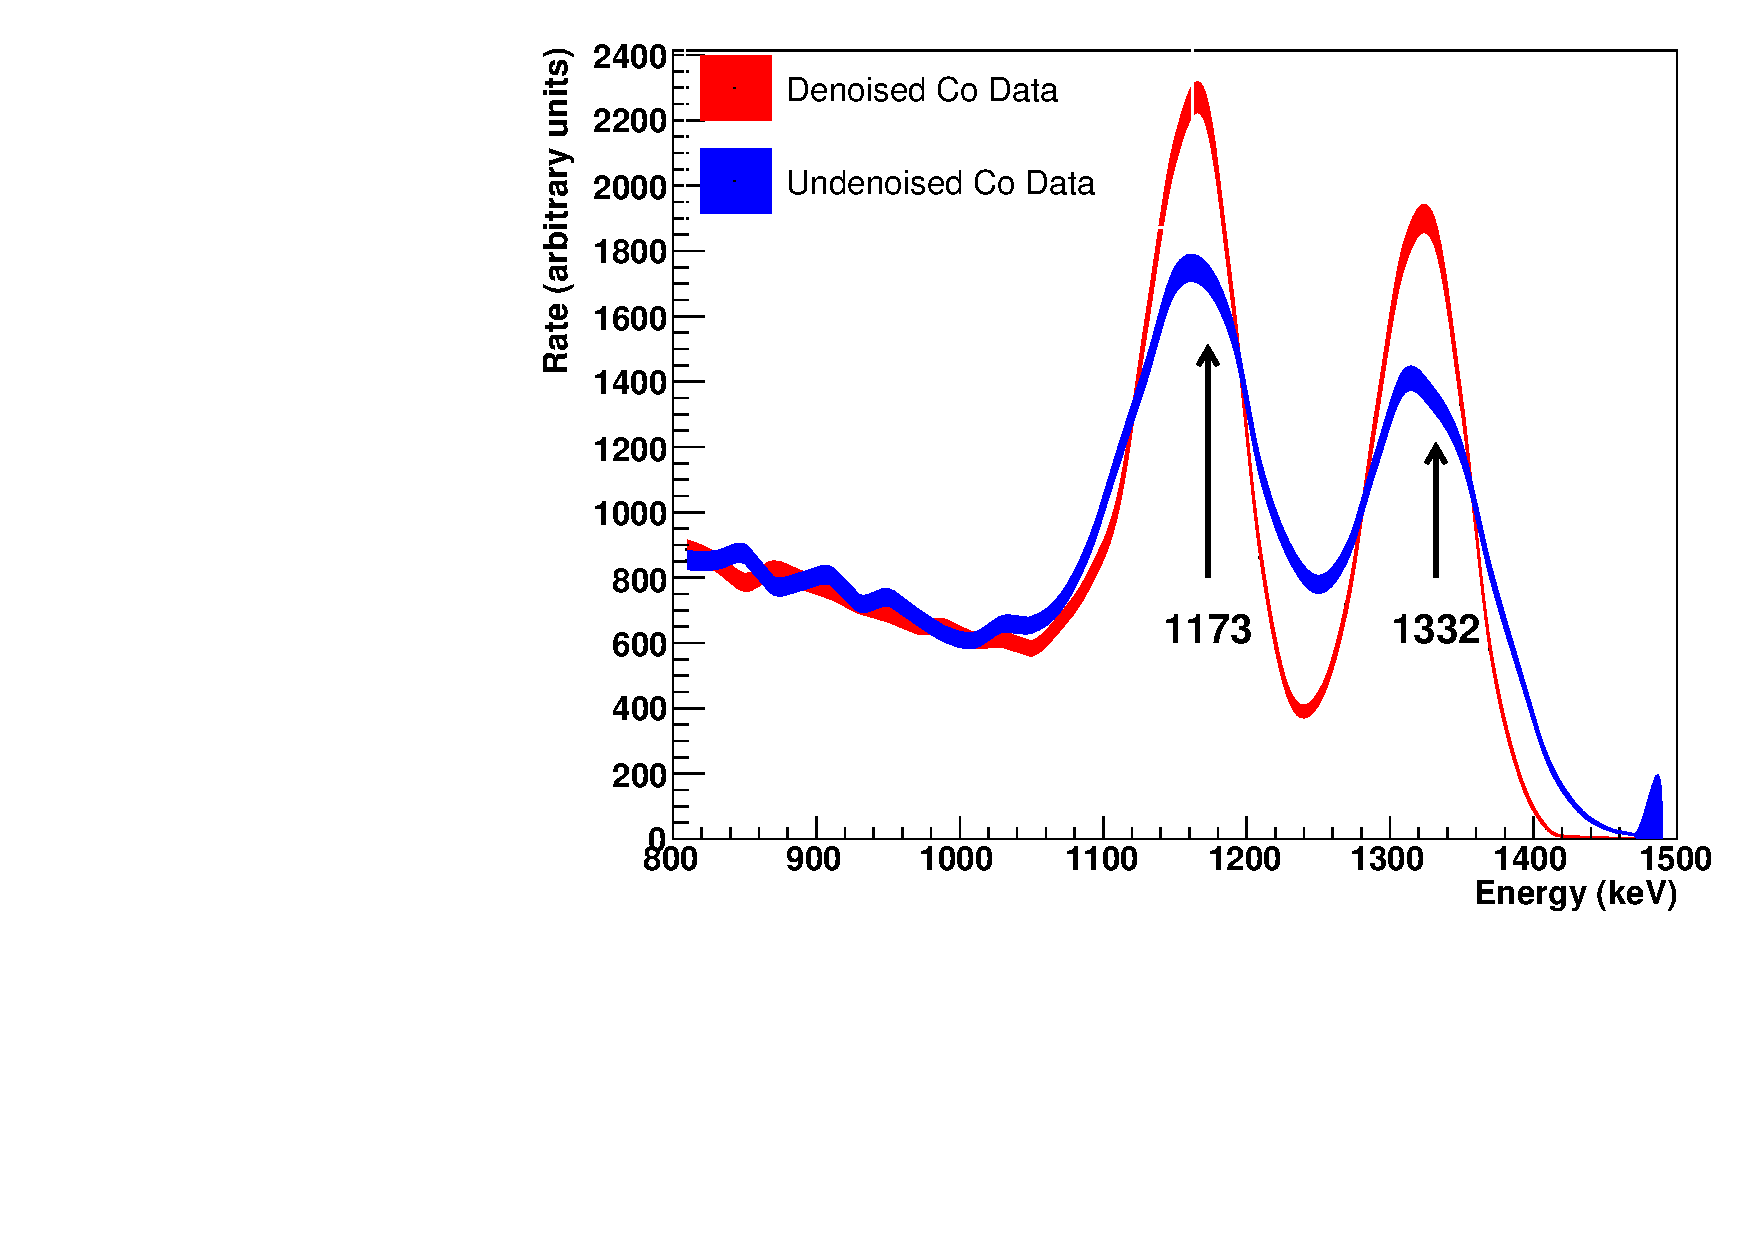
\includegraphics[keepaspectratio=true,width=\textwidth]{CoSourceSpectrumComparison.pdf}
\end{center}
\end{frame}

\begin{frame}
\begin{center}
\frametitle{$^{137}$Cs Source Spectrum (Before and After)}
\end{center}
\vspace{1cm}
\begin{center}
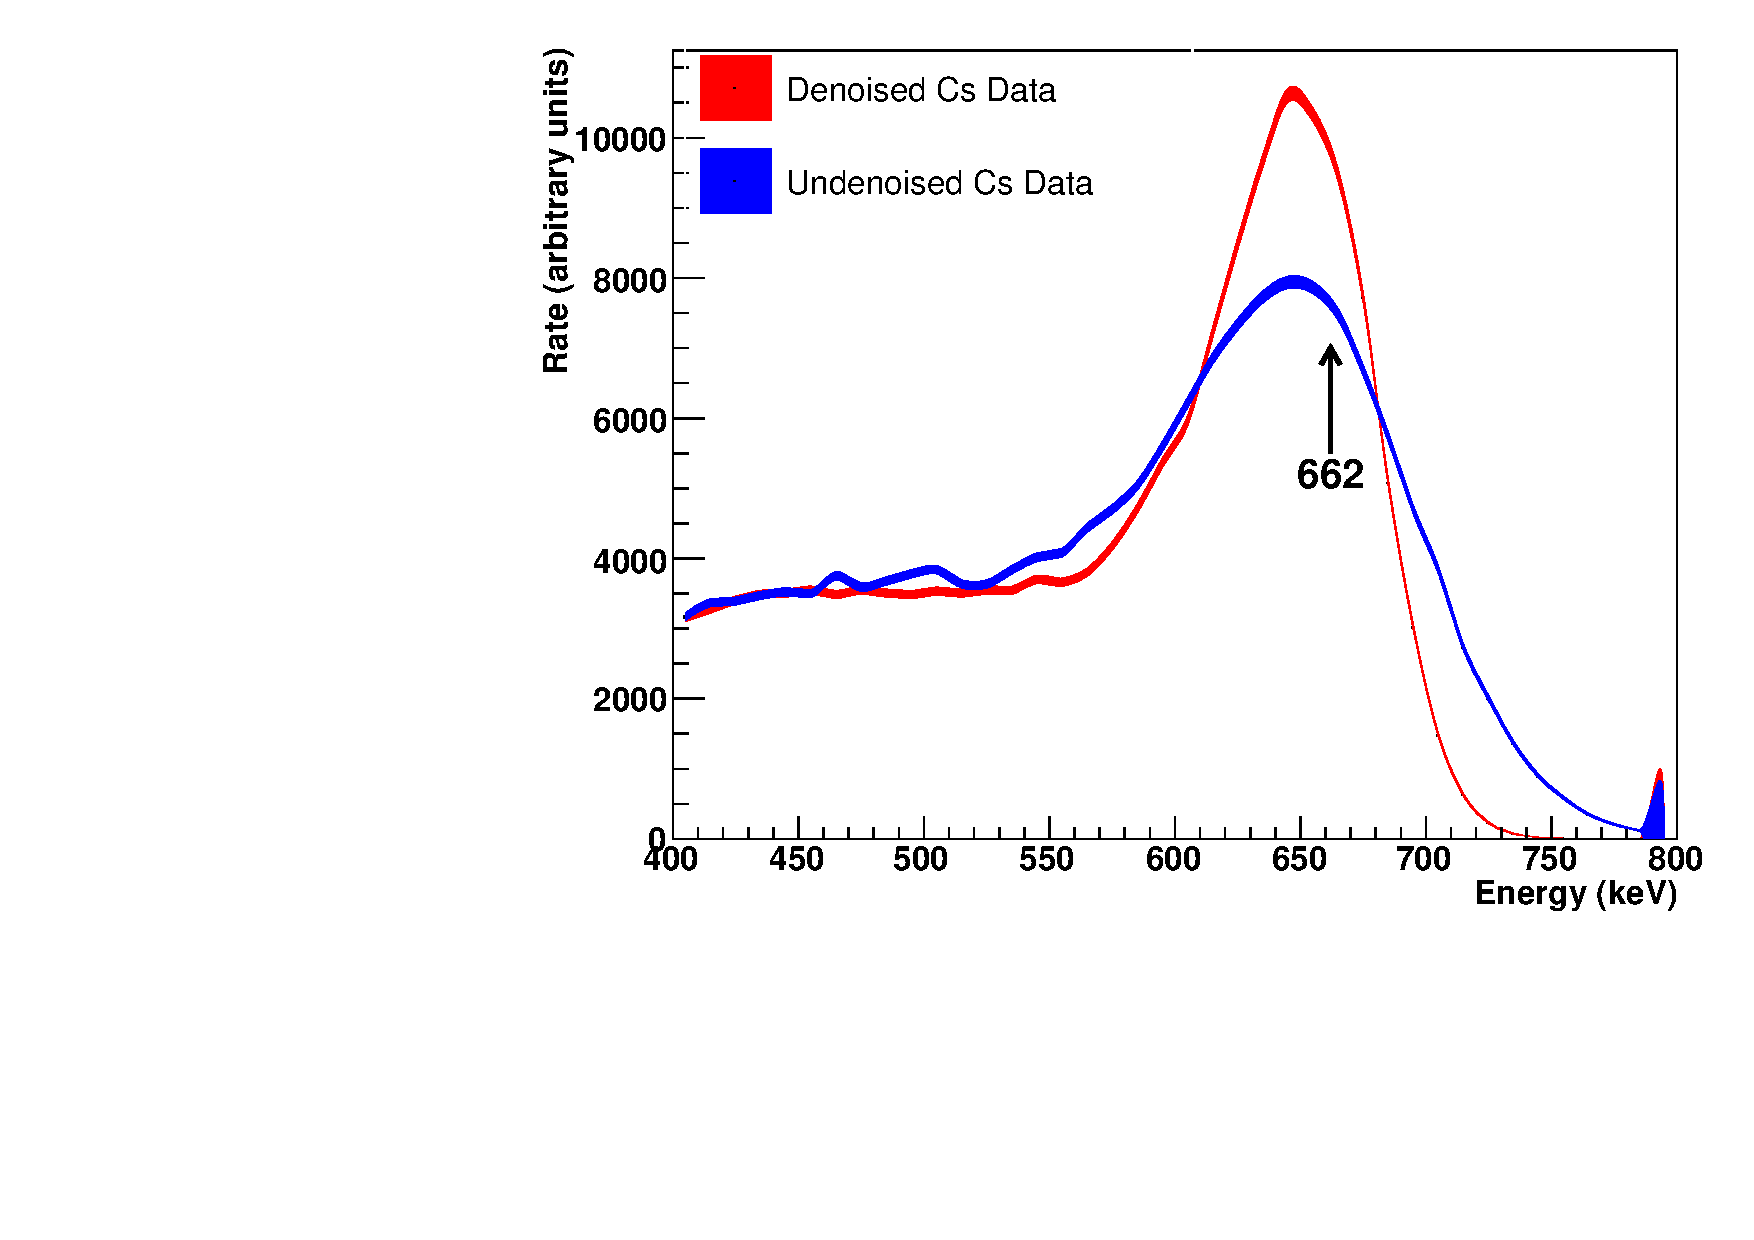
\includegraphics[keepaspectratio=true,width=\textwidth]{CsSourceSpectrumComparison.pdf}
\end{center}
\end{frame}

\begin{frame}
\begin{center}
\frametitle{Energy Resolution (Before and After)}
\end{center}
\vspace{0.6cm}
\begin{center}
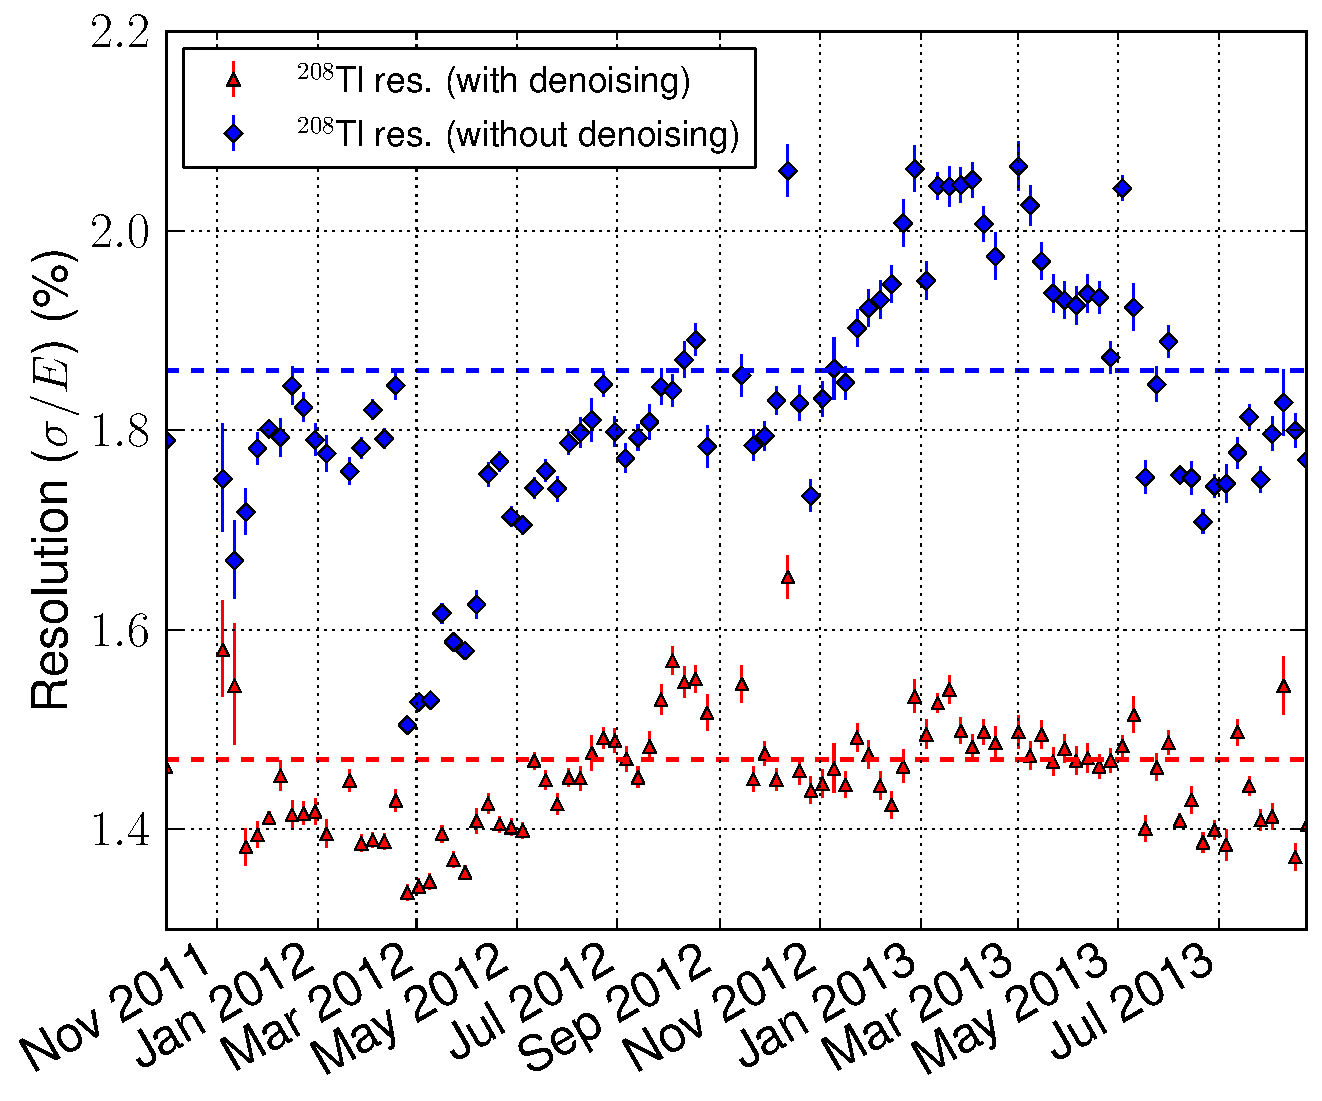
\includegraphics[keepaspectratio=true,width=.95\textwidth]{RotatedReso_denoised_compVsTime.pdf}
\end{center}
\end{frame}

\begin{frame}
\begin{center}
\frametitle{Energy Resolution (Before and After)}
\end{center}
\vspace{0.5cm}
\begin{center}
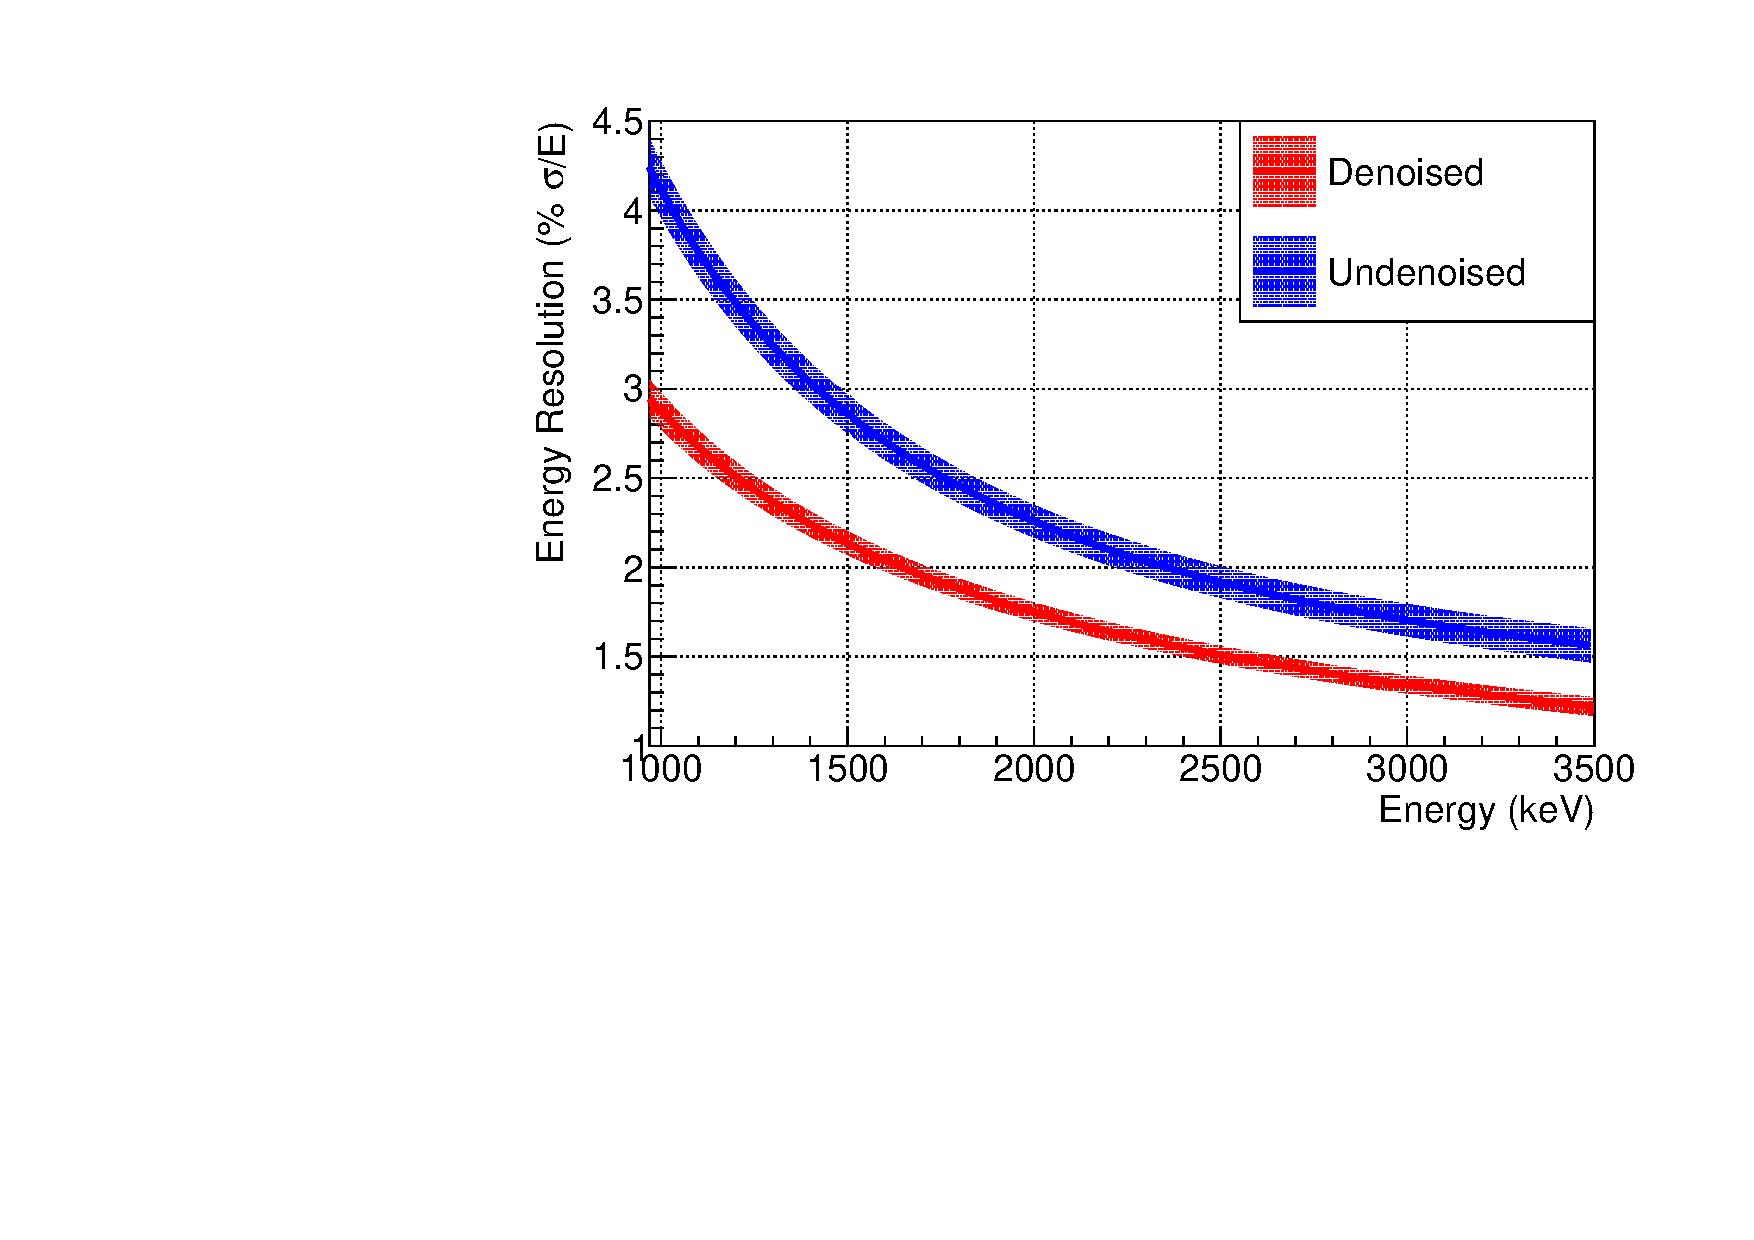
\includegraphics[keepaspectratio=true,width=\textwidth,clip=true,trim=0mm 0mm 10mm 10mm]{ResolutionFunctionComparison_relative.pdf}
\end{center}
\end{frame}

\begin{frame}
\begin{center}
\frametitle{Best Fit (Denoised)}
\end{center}
\vspace{0.6cm}
\begin{center}
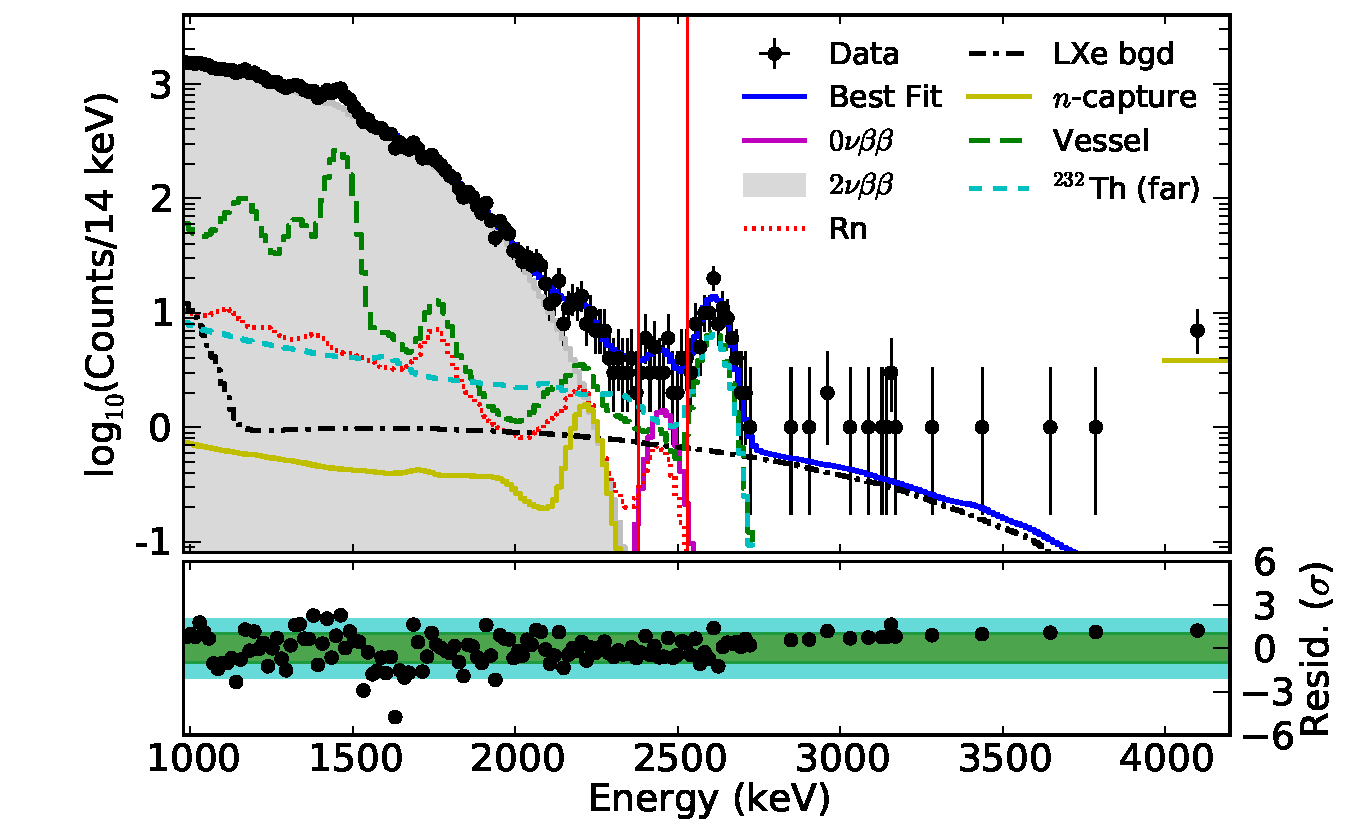
\includegraphics[keepaspectratio=true,width=\textwidth,clip=true,trim=14mm 0mm 0mm 0mm]{Energy_BestFit_ss.pdf}
\end{center}
\end{frame}

\begin{frame}
\begin{center}
\frametitle{Best Fit (Denoised), multi-site backgrounds}
\end{center}
\vspace{0.6cm}
\begin{center}
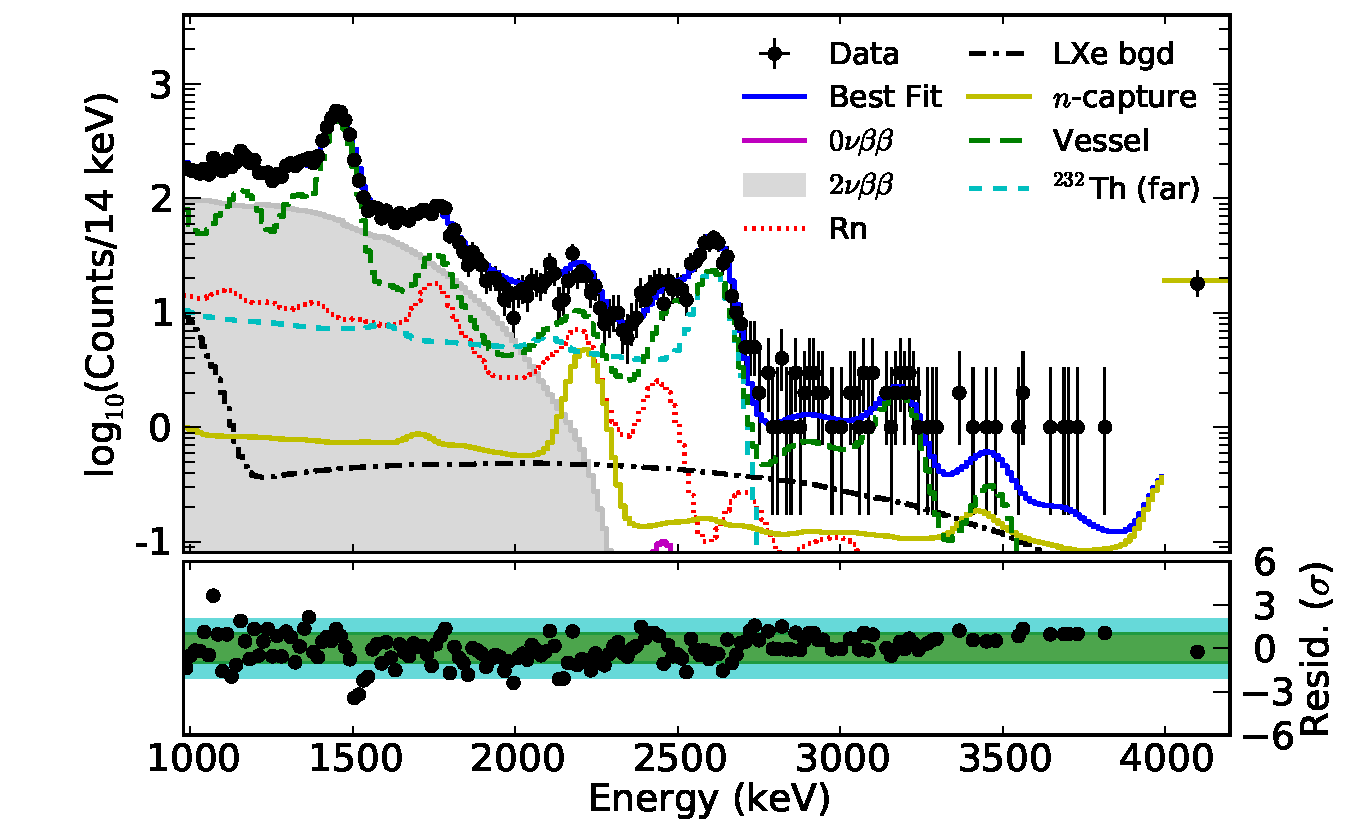
\includegraphics[keepaspectratio=true,width=\textwidth,clip=true,trim=14mm 0mm 0mm 0mm]{Energy_BestFit_ms.pdf}
\end{center}
\end{frame}

\begin{frame}
\begin{center}
\frametitle{Fits around $\beta \beta 0\nu$ (Before and After)}
\end{center}
\vspace{0.6cm}
\begin{center}
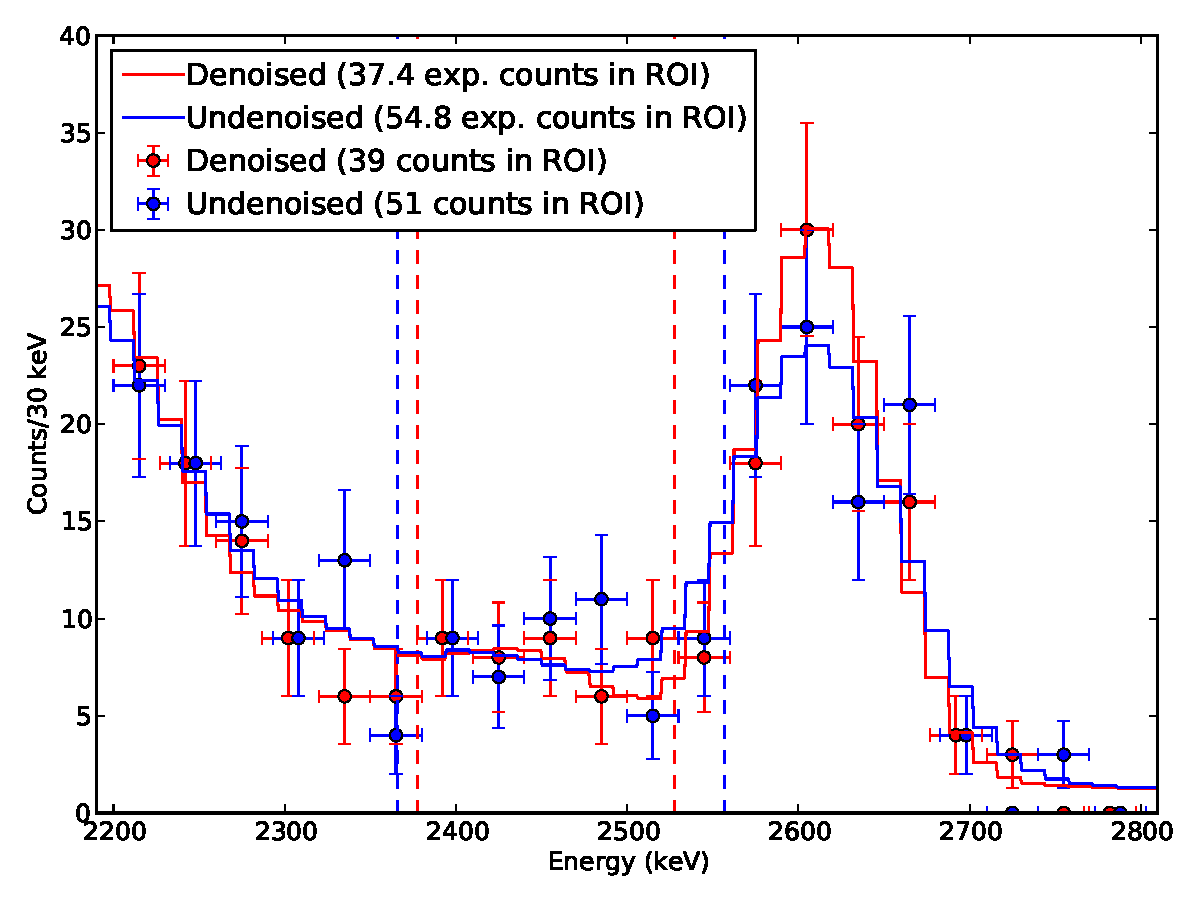
\includegraphics[keepaspectratio=true,width=\textwidth]{DenoisedVsUndenoised_TotalPdfsWithData.pdf}
\end{center}
\end{frame}

\begin{frame}
\begin{center}
\frametitle{Profile Likelihood (Before and After)}
\end{center}
\vspace{0.6cm}
\begin{center}
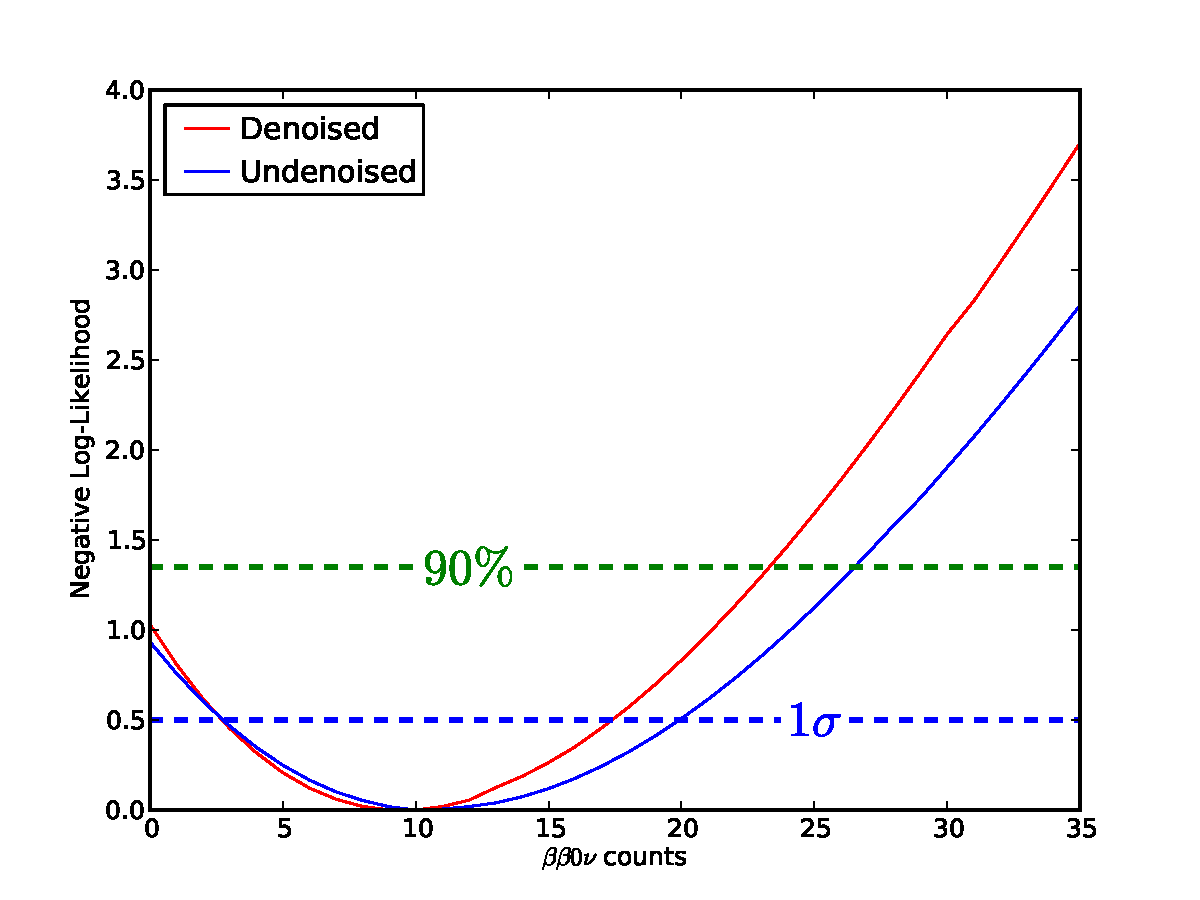
\includegraphics[keepaspectratio=true,width=\textwidth]{DenoisedVsUndenoised_bb0nProfiles.pdf}
\end{center}
\end{frame}

\begin{frame}
\begin{center}
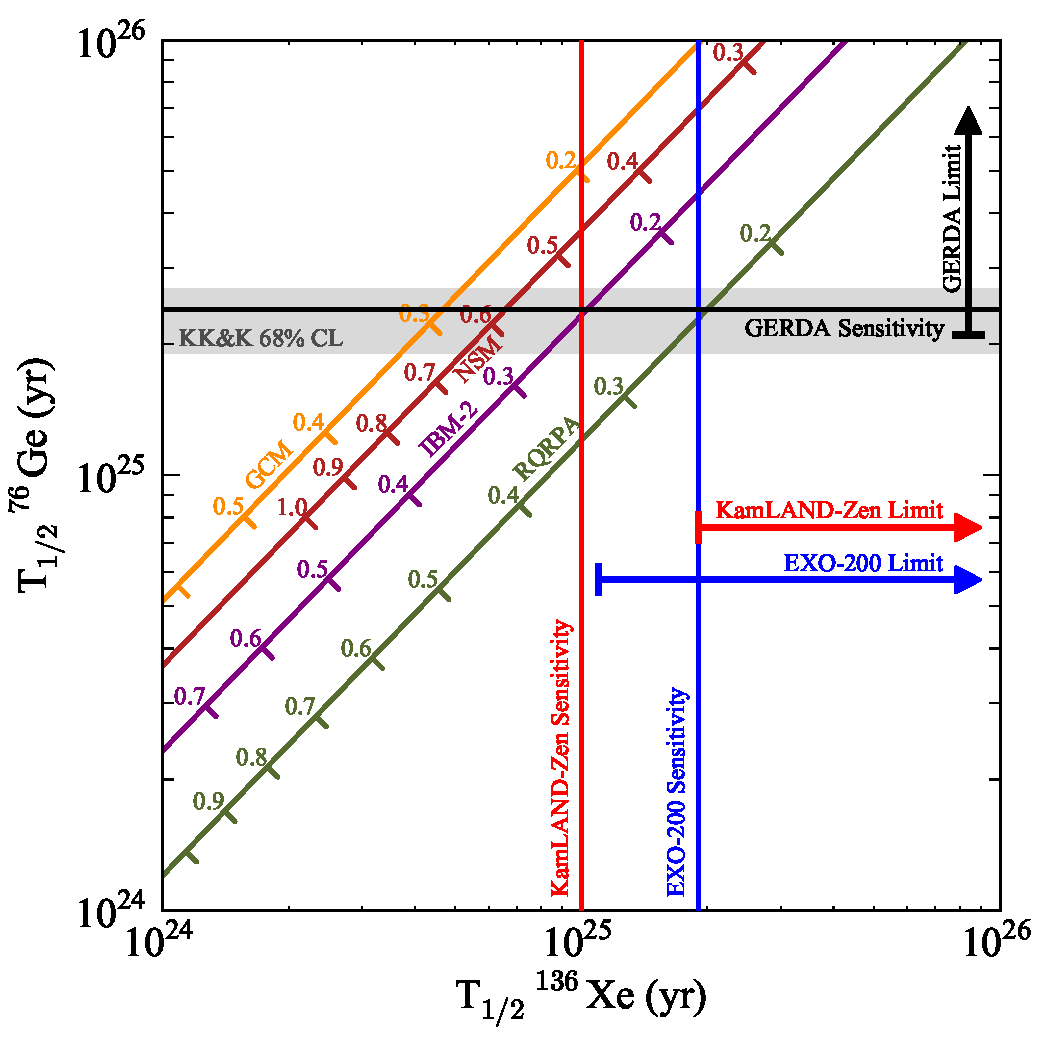
\includegraphics[keepaspectratio=true,width=3.7in]{MatplotLibSensitivity.pdf}
\end{center}
\end{frame}

\begin{frame}
\begin{center}
\frametitle{The EXO-200 Collaboration}
\end{center}
\vspace{0.5cm}

{\tiny
\textcolor{red}{University of Alabama, Tuscaloosa AL, USA}  -  D. Auty, T. Didberidze, M. Hughes, A. Piepke, R. Tsang\\
\textcolor{red}{University of Bern, Switzerland}  -  S. Delaquis, G. Giroux, R. Gornea, T. Tolba, J-L. Vuilleumier \\
\textcolor{red}{California Institute of Technology, Pasadena CA, USA}  -  P. Vogel \\
\textcolor{red}{Carleton University, Ottawa ON, Canada}  -  V. Basque, M. Dunford, K. Graham,  C. Hargrove, R. Killick, T. Koffas, F. Leonard, C. Licciardi, M.P. Rozo, D. Sinclair\\
\textcolor{red}{Colorado State University, Fort Collins CO, USA}  -  C. Benitez-Medina, C. Chambers, A. Craycraft, W. Fairbank, Jr., T. Walton\\
\textcolor{red}{Drexel University, Philadelphia PA, USA}  -  M.J. Dolinski, M.J. Jewell, Y.H. Lin, E. Smith, Y.-R Yen\\
\textcolor{red}{Duke University, Durham NC, USA}  -  P.S. Barbeau\\
\textcolor{red}{IHEP Beijing, People's Republic of China}  -  G. Cao, X. Jiang, L. Wen, Y. Zhao \\
\textcolor{red}{University of Illinois, Urbana-Champaign IL, USA}  -  D. Beck, M. Coon, J. Ling, M. Tarka, J. Walton, L. Yang \\
\textcolor{red}{Indiana University, Bloomington IN, USA}  -  J. Albert, S. Daugherty,  T. Johnson, L.J. Kaufman\\
\textcolor{red}{University of California, Irvine, Irvine CA, USA}  -  M. Moe\\
\textcolor{red}{ITEP Moscow, Russia}  -  D. Akimov, I. Alexandrov, V. Belov, A. Burenkov, M. Danilov, A. Dolgolenko, A. Karelin, A. Kovalenko, A. Kuchenkov, V. Stekhanov, O. Zeldovich\\
\textcolor{red}{Laurentian University, Sudbury ON, Canada}  -  B. Cleveland, A. Der Mesrobian-Kabakian, J. Farine, B. Mong, U. Wichoski\\
\textcolor{red}{University of Maryland, College Park MD, USA}  -  C. Davis, A. Dobi, C. Hall \\
\textcolor{red}{University of Massachusetts, Amherst MA, USA}  -  J. Abdollahi, T. Daniels, S. Johnston, K. Kumar, A. Pocar, D. Shy\\
\textcolor{red}{University of Seoul, South Korea}  -  D.S. Leonard\\
\textcolor{red}{SLAC National Accelerator Laboratory, Menlo Park CA, USA}  -  M. Breidenbach, R. Conley, A. Dragone, K. Fouts, R. Herbst, S. Herrin, A. Johnson, R. MacLellan, K. Nishimura, A. Odian, C.Y. Prescott, P.C. Rowson, J.J. Russell, K. Skarpaas, M. Swift, A. Waite, M. Wittgen\\
\textcolor{red}{Stanford University, Stanford CA, USA}  -  J. Bonatt, T. Brunner, J. Chaves, J. Davis, R. DeVoe, D. Fudenberg, G. Gratta, S.Kravitz, D. Moore, I. Ostrovskiy, 
A. Rivas, A. Schubert, D. Tosi, K. Twelker, M. Weber\\
\textcolor{red}{Technical University of Munich, Garching, Germany}  -  W. Feldmeier, P. Fierlinger,  M. Marino\\
\textcolor{red}{TRIUMF, Vancouver BC, Canada} – J. Dilling, R. Krucken, F. Reti\`ere, V. Strickland\\
}

\end{frame}

\begin{frame}
\begin{center}
{\Huge Thank You!\\[\baselineskip]

Questions?}
\end{center}
\end{frame}

% What does it mean that our optimization problem is positive-definite before the constraint is imposed, but not after?  Are we actually not getting an optimal solution??

% What does 90% confidence mean for us?  Review (in the fitting document) exactly what hypothesis we're testing when we talk about coverage.

%%%%%%%%%%%%%%%%%%%%%%%%%%%%%%%%%%%%%%%%%%%%%%%%%%%%%%%%%%%%%%%%%%%%%%%%%%%%%%%

\begin{frame}
\frametitle{Backup Slides}
\end{frame}

\begin{frame}
\begin{center}
\frametitle{Anticorrelated Scintillation/Charge}
\end{center}
\vspace{.5cm}
\begin{center}
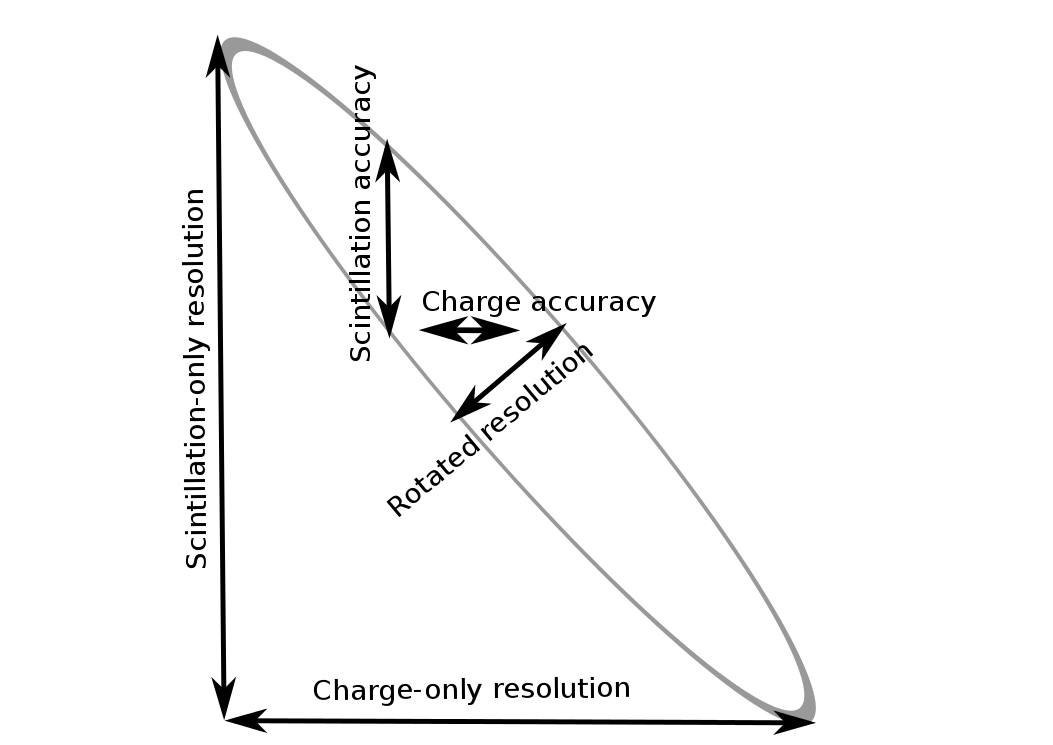
\includegraphics[keepaspectratio=true,width=\textwidth]{RotatedIsland.png}
\end{center}
\end{frame}

\begin{frame}
\begin{center}
\frametitle{Why not the Anscombe transformation?}
\end{center}
The Anscombe transformation (and generalizations) are designed to transform Poisson noise into Gaussian noise.  However, for this purpose ``noise'' is defined to mean noise {\bf uncorrelated with pulse}.  We, on the other hand, are looking to understand noise which {\bf is} correlated with the pulse, and then minimize its effect.

So, the Anscombe transformation doesn't really help us here.
\end{frame}

\begin{frame}
\begin{center}
\frametitle{Impact of Rotated Energy}
\end{center}
\begin{center}
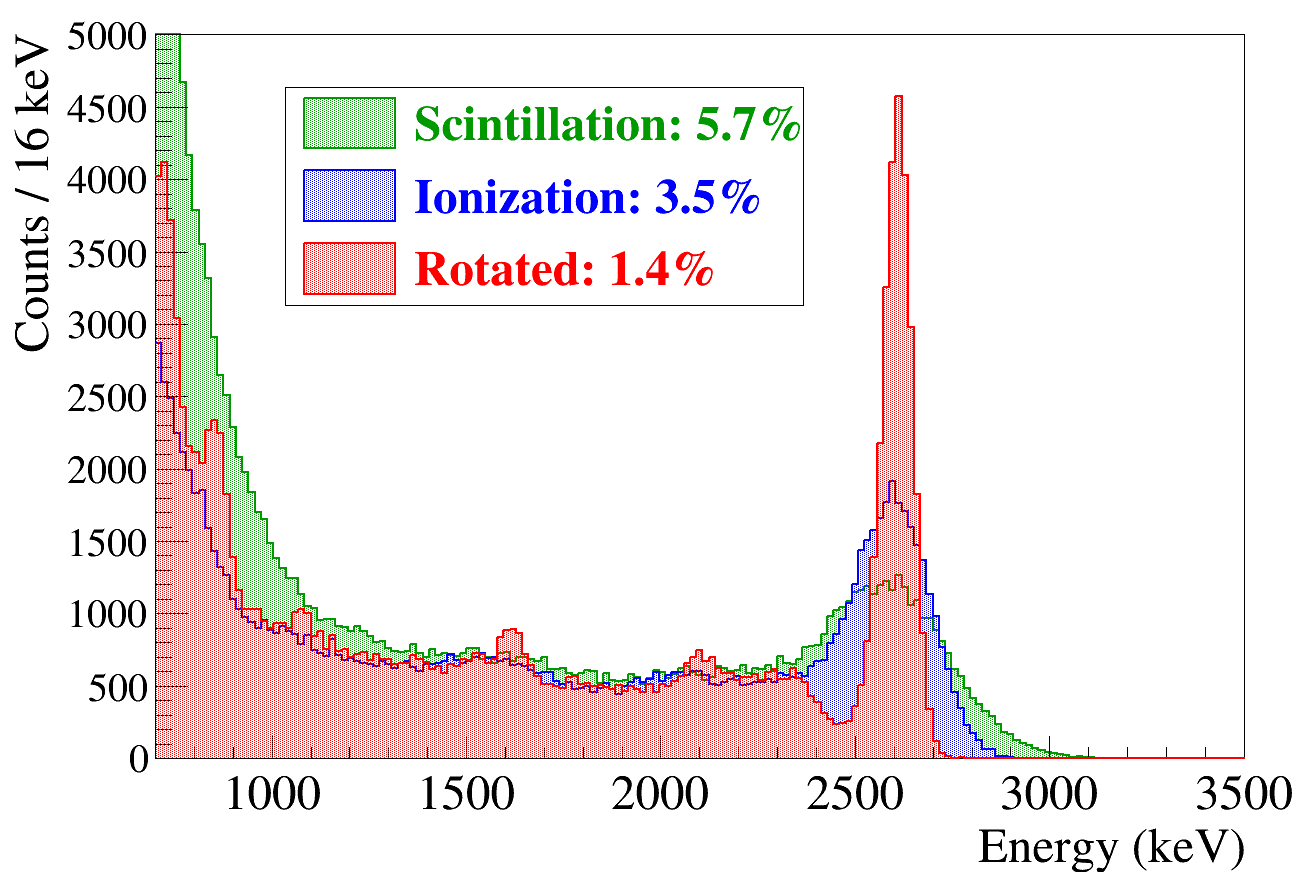
\includegraphics[keepaspectratio=true,width=\textwidth]{RotationTh2D_ImprovementInResolution.png}
\end{center}
\end{frame}

\begin{frame}
\begin{center}
\frametitle{Energy Resolution (Before and After)}
\end{center}
\vspace{0.5cm}
\begin{center}
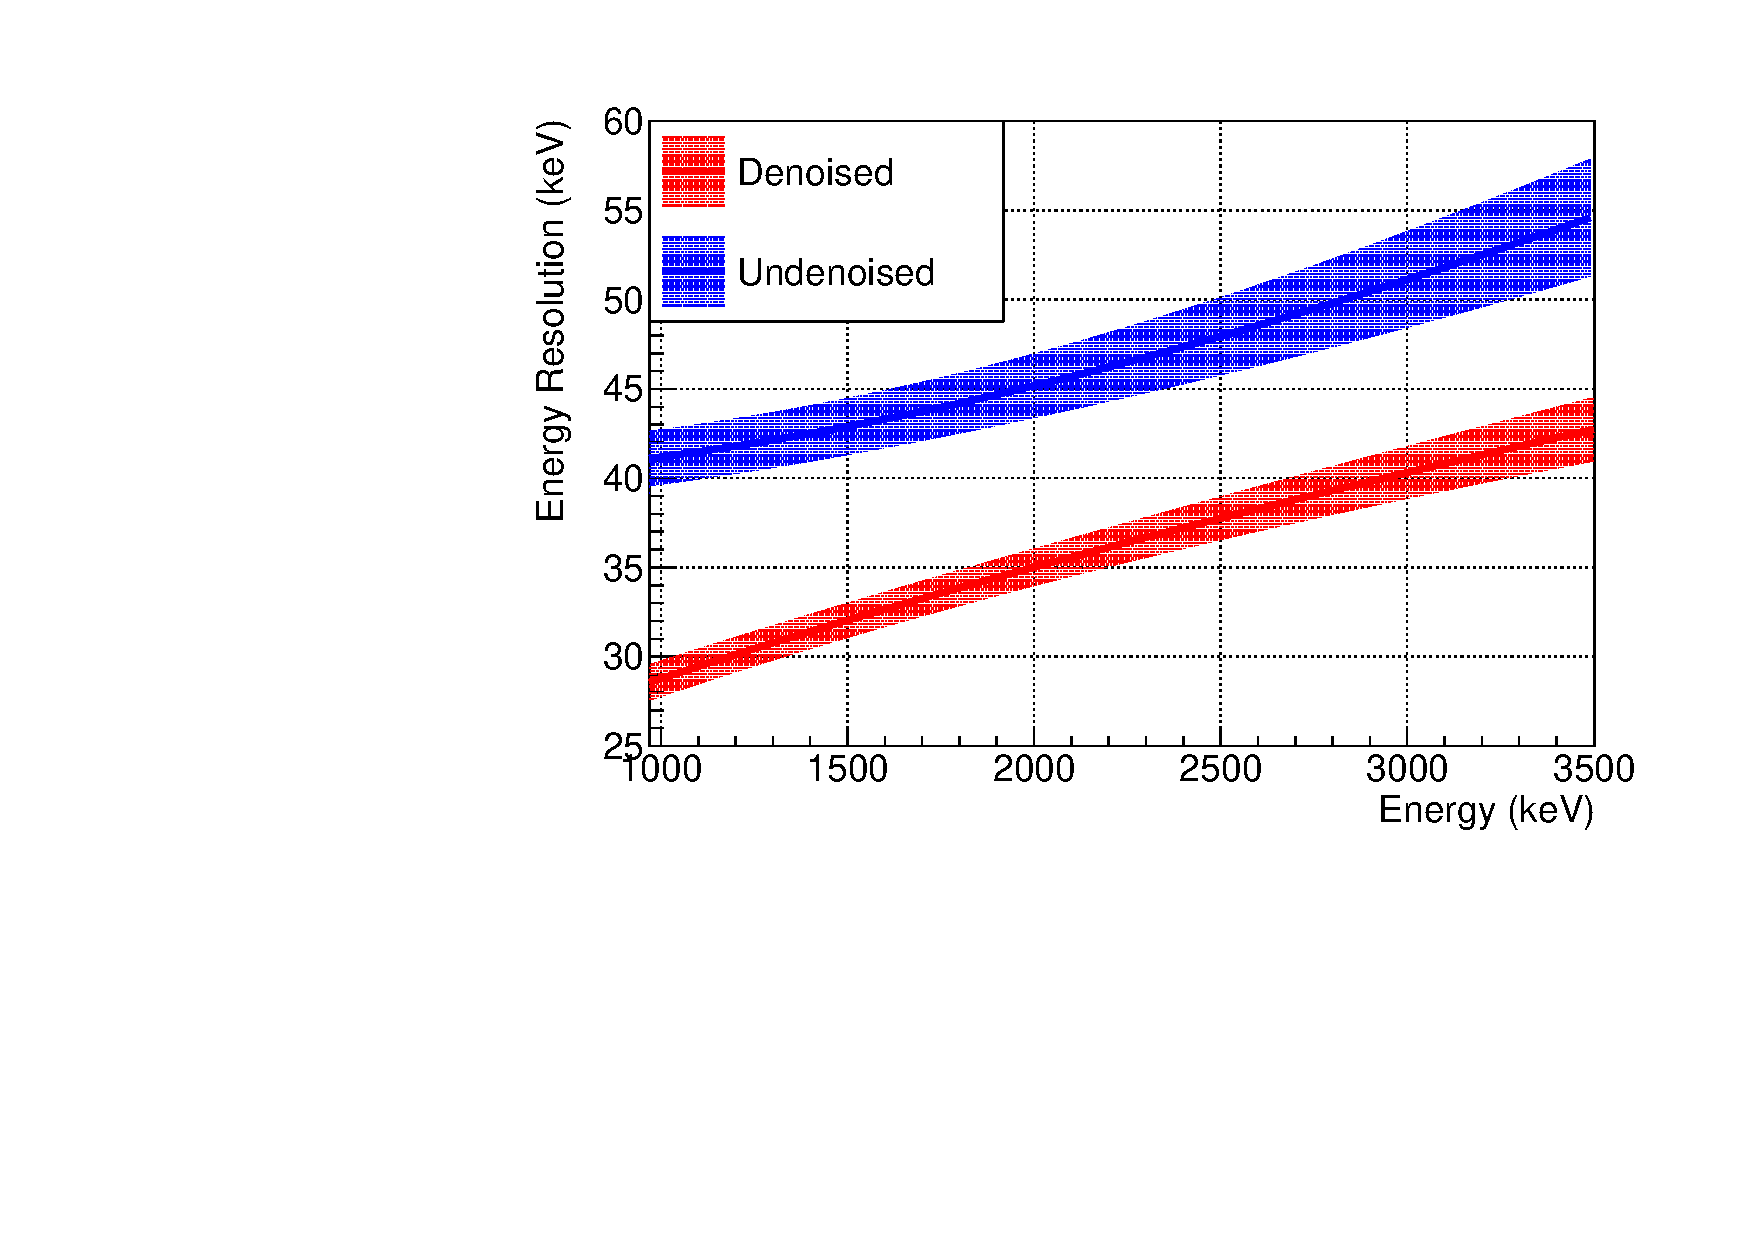
\includegraphics[keepaspectratio=true,width=\textwidth,clip=true,trim=0mm 0mm 10mm 10mm]{ResolutionFunctionComparison_absolute.pdf}
\end{center}
\end{frame}

\begin{frame}
\begin{center}
\frametitle{Mean Sensitivity}
\end{center}
\vspace{0.6cm}
\begin{center}
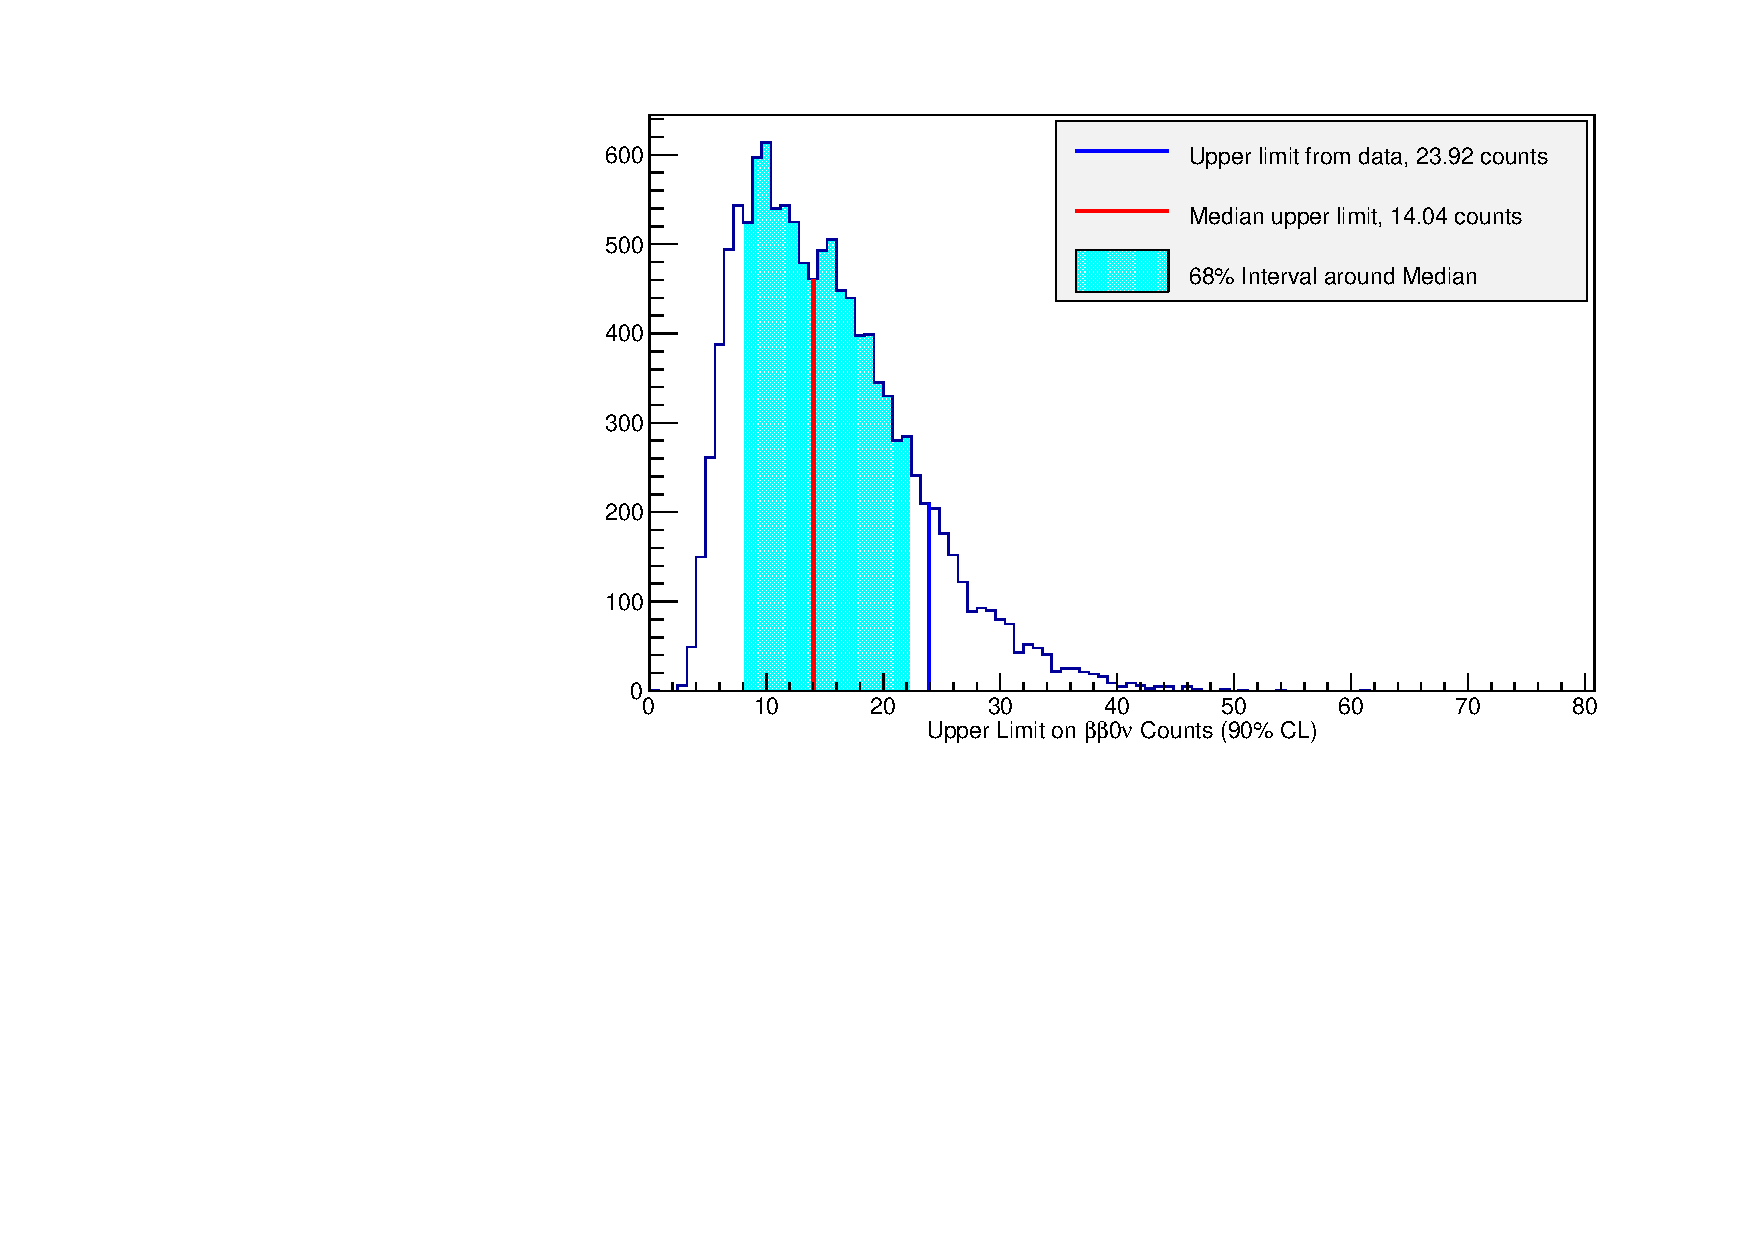
\includegraphics[keepaspectratio=true,width=\textwidth]{toy_mc_sensitivity.pdf}
\end{center}
\end{frame}

% X-ray attenuation
% SS/MS (If I don't address it directly.)
% Alpha discrimination.
% Muon-vetoed spectrum.
% Sensitivity.
% More spectra.
% Denoised vs non-denoised spectra from individual background components.

\end{document}

